\documentclass[a4paper,11 pt]{article}

\usepackage[utf8]{inputenc}
%\usepackage[T1]{fontenc}
%\usepackage{babel}
\usepackage{graphicx}

\usepackage[font=small,format=plain,labelfont=bf,up,textfont=it,up]{caption}

\usepackage{amsmath}
\usepackage{mathrsfs} %brukt for krølle-L : laplace


\author{Per R. Leikanger}
                             
\title{Project}
\date{\today}     

%\usepackage{natbib}    Kva er dette? Er med i rapport 3002.

\begin{document}   

\maketitle

\tableofcontents

\newpage

% KAPTITTEL : Introduction
%TODO Må skrives: sett av 0.7 dag til dette.

%Todo Skriv kvifor eg 'cite' kapittel til de ulike bøkene. Bøkene er ofte så store at uten dette blir referansene memingsløs..




%
% 	- Utvida innholdsfortegnelse.
% 	- Skrive at eg har, og vise til kor eg har    ->  svart på de ulike aspektene ved oppgaveteksten.
% 	- Skrive eksplisitt om oppgaveteksten.
% 	- 
% 	- 

\newpage
\section{Oppgavetekst}
In most artificial neural networks (ANN),  a neuron's output variable can be said to represent the time varying firing rate (i.e. number of action potentials per time unit) of its biological equivalent.\\
In this domain, there is no representation of firing time and other aspects related to causality and stability that appear to be central to the learning process in a biological neural network.
 
 In this project, you will develop a new concept for ANN that takes into consideration both firing rate and firing time, and compare it with the existing model known as Spiking ANN (SANN).
 \begin{itemize} 
  \item[1] Give an overview of existing ANN models that represents both firing rate and firing time. Emphasis should be put on factors that can be related to stability for synaptic plasticity (learning) and/or feedback ("recurrent ANN").
  \item[2] Describe the new ANN concept, and point out how this differs qualitatively from previous models.
  \item[3] Compare the new concept with competing methods. The evaluation may be based on a number of specific scenarios (with respect to input data etc.).
 \end{itemize}

 Supervisor:      Øyvind Stavdahl, Associate Professor, Department of Engineering Cybernetics, NTNU\\
                  Professor Gaute Einevoll, Department of Mathematical Sciences and Technology, Norwegian University of Life Sciences.
\newpage

\section{Abstract}
Husk: tittel er ekte delmengd av abstract, som er ekte delmengd av introduction, som er ekte delmengd av rapport.

\section{Introduction}

In this text many 

% XXX Følgende er kjempeviktig å ha med:
In this report the convention used by Rolls and Treves in ``Neural Networks and Brain Functions'' will be used. 
For any transmission through a synapse between neuron $j$ and neuron $i$, we define the synaptic strength $w_{ij}$.  % TODO Skriv heller: "..through a synapse FROM neuron $j$ TO neuron $i$, we .."
Note that the first subscript refers to the recieving neuron and the last subscript to the presynaptic neuron (the signalling neuron) \cite{TrevesNeuralNetworks}.
This convention will be used in this text. 
% XXX XXX XXX  (bra skrevet er det og)






%TODO NEVN action potential i innledning! XXX VIKTIG!




%(tidligere) KLADD:
%Recently, there have been a strong focus on the timing of spikes. There are two reasons behind this.
%The first is connected to synaptic plasticity. 
%In 1987, Gustavsen et. al. found that synaptic plasticity could vary as a function of the postsyn
%Synaptic plasticity can be divided in two groups, Long Term Potentiation (LTP) causing an a lasting increase in the synaptic weight and Long Term Depression (LTD) causing a lasting decrease in the synaptic weight.
%Gustavsen et. al found in 1987 that the synaptic plasticity vas a function of the postsynaptic depolarization at the time of transmission. 
%The synaptic plasticity varied from a strong LTP to a strong LTD as a result from a single transmission\cite{Gustafsson03011987}.
%%Dette ble også overført til ANN

%We can say that, statistically there is a correlation between the presynaptic depolarization after a synaptic transmission, and the relative timing of the postsynaptic action potential. %ELLER NOKE: RYDD OPP XXX XXX
%If we view this statistically, we can say that the timing of the presynaptic action potential (``firing'') in relation to the postsynaptic firing is a direct consequence of the postsynaptic potential at the time of transmission.
%Based on this analysis alone, we can say that the relative timing of the pre-- and post-- synaptic firing is fundamental for the size and direction of the synaptic plasticity.
%% XXX KVIFOR tidavhengig? XXX : There are also hypothesis about a retrograde signalling mechanism in the neuron that gives the same effect
%This recieved the name ``Spike Time Dependent Plasticity''(STDP).








%TODO Skriv at eg kaller implementasjonen for AuronSim, og dette navnet vil opptre under mange av kurvene i rapporten.


%todo todo todo Skriv kvifor eg har så mykje neuro-info: dette kan sees på son en del av utviklingsprosessen: det å lære om neuronet er viktig for å skrive en simulator av dette..

% Skrive at denne teksten er laget som resultat av arbeidet mitt.
% I mange tilfeller der det ikkje er referanser er dette fordi eg ikkje har basert denne delen av arbeidet på andres arbeid, men utvikla det selv. 
% 	Dette gjelder spesielt for SANN modellen min, siden eg begynte dette arbeidet før eg i det heile tatt viste at det fantes noko som var kalla SANN. Mangler på referanser er dermed selvfoklart. 
% 	Eg har i desse tilfeller prøvd å få med store deler av utviklingsprosessen.
%
% For KANN har eg enda ikkje funnet andre modeller basert på desse ligningene, og er fortsatt av den tro at dette er nytt arbeid.
% 	For KANN har eg difor alltid vist utviklignsprosessen for både modellen og impelmentasjonen. Dette ble mye tekst, men dette er eit resultat av mangler på kilder å henvise til.
%
% Før eg kan begynne å snakke om SANN modellen eller KANN modellen trenger eg å etablere eit felles utgangspunkt for forfatteren og leseren. 
% 	Dette er forsøkt gjordt ved å ha en grundig gjennomgang av ANN og det biologiske systemet,tidlig i teksten(i kap. 1). Supplerende informasjon og informasjon som faller utenfor oppgaven er plassert i appendix, og er også egenprodusert.
% 	
% Kap. 2 er forbeholdt modellering av neuronet, og for innføring i bakgrunnsmatematikken som ligger bak den nye modellen.
% 	Det er godt mulig at resultatene fra dette kapittelet også kan være til bruk for neuralscience, da det gjør eit forsøk på å etablere bedre fremgangsmåter for "aktivitetsvariabler" for neuronet. 
% 	Den gjeldende aktivitetsvariabelen for neuron er basert på fyringsraten til neuronet, noko som ikkje er særlig intuitivt med tanke på "instataneouis firing rate". Den nye modellen opner for umiddelbare aktivitetsvariabler.
%
% 	I de to første kapittel er mesteparten av bakgrunnsinformsjonen presentert, så mesteparten av 'citations' vil finnes her. Seinere kapittel vil inneha ferre 'citations', da dette i all hovedsak er basert på eget arbeid.
% 		XXX Kanskje dette ikkje stemmer for Kap 3? Veit ikkje enda, siden det ikkje er skrevet. Trur ikkje det..
%
% Kap. 3 Omhandler design og implementasjon av de ulike modellene. 
% 	Section {ref:design} handler om den generelle strukturen for implementasjonane. Her beskrives flere metoder for å gjøre implementasjonene mest mulig sammenlignbar for denne oppgaven.
% 		Resultat presentert i kapittel 1 vil være viktig i dette kapittelet, siden implementasjonene er prøvd å gjøres lik det biologiske systemet. 
% 		Den modulære oppbyggingen til det kunstige neuronet (auronet) er beskrevet og  vil være gjeldende for begge modellene.
% 		Element som object design og metoder for effektivisering vil bli presentert.
% 		I tillegg vil en "to my knowledge" ny modell for tid bli presentert. Denne modellen er viktig for begge modellene, siden den gir oss mulighet for å ha simulert asynkronitet for nodene i neuralnettet.
% 		Logg. pCalculationTaskQue, pWorkTaskQue?, ...
% 	Section {ref:SANN-imp} handler om design og implementasjon av SANN
% 		Dette kapittelet går gjennom mekanismene som ligger bak simulering av mitt SANN. Dette kapittelet lener seg sterkt på element presentert i kapittel 1 og litt fra kap. 2.
% 		Modellen er egenprodusert, selv om den tidligere har blitt etablert (REFER til når/kor/kven). Dette dobbeltarbeidet er en konsekvens av manglende kunnskap for kildesøk når eg studerte neuro.
% 		Section {SANN-imp} avaluttes med en utskrift (plot) laget ved en kjøring av SANN simulatoren.
% 	Section {ref:KANN-imp}
%  		Dette kap. begynner med å beskrive konsept som må behandles ulikt fra det som er presentert i section {SANN-imp}. 
% 		Siden modellene er basert på heilt fremgangsmåter for å simulere eit LIF neuron, begynner forskjellene allerede ved aktivitetsvariabelen.
% 			For SANN er artivitetsvariabelen en etterligning av det biologiske neuronets aktivitetsvariabel, det elektriske potensialet over membranen. 
% 			For KANN er aktivitetsvariabel basert på resultat fra kap. 2, som er, så vidt eg veit, en heilt ny måte å modellere neuronets aktivitet på.
% 		Dette skaper også ulikheter i korleis aktivitet propagerer gjennom systemet. Mykje av det resterende i section{KANN-imp} er brukt på dette.
% 		Mot slutten diskuteres metoder for å gjøre KN kompatibel med SN, spesielt i retninga KN->SN. 
% 		Section{KANN-imp} avsluttes med en diskurs om når Kappa bør propagere videre til neste noder. Dette er eit viktig element og (BØR) dekkes grundig. TODO Dekk grundig!
% 		%KANSKJE lag eit plott som ligner på plottet i {SANN-imp} og skriv at kapittel avsluttes med samme som {SANN-imp}.
% Kap 4 er avsatt sammenligning og resultat av prosjektet. TODO Skriv dette etter at eg har skrevet Kap 4 XXX
%
%
%
%
% 	Aspekter ved oppgaven / kor er det besvart?
% 		Sammenligning: skriv at eg desverre ikkje fekk tid å sammenligne effektivitet, så denne tolkningen av oppgaven må vente til senere.
%
%
%
%





















% 	- 
% 	- 
% OPPSETT:
% 	- Oppgaveteksten.
% 	- Tolke oppgaveteksten (skriv at ".." tolkes som ?, og kan analyse av dette kan finnes i section \ref{}
% 	- Skrive at fokus kan være pragmatisk eller simulativt, for ANN. Eg har prøvd å lage min implementasjon så generell som mulig (dvs. at den er laget med et fokus på å kunne lett utvides til å være meir egna til simulering av NN).
% 	 	I tillegg har eg fukusert på å lage det likest mulig biologien. Dette er siden kvart generasjonsskifte i ANN, i tillegg til å bli bedre (med ulike vekter for "bra"), så har det også nerma seg biologien. Meir i kap. ANN.
% 	- Relevant bakgrunnsinfo om biologiske system er dermed gått gjennom i "BiologiskeSystemet".
% 		Dette blir formalisert matematisk og modellert i section "theNewModel".
% 	- Derretter gjennomgåes design og implementasjon av simulatoren i kap. "design", implementasjon_SANN og implementasjon_KANN.
% 		Dette for å seinere kunne analysere forskjellene mellom de to modellene for implementasjon av pulsed neural networks.
% 	- I kap. "metodeForSammenligning.tex" går vi også gjennom andre sammenligninger mellom de to implementasjonene.
%
% 	Rapporten blir avsluttet med en oppsummering og tolking av sammenligningene gjort i denne rapporten. (Sjå resultat.tex for meir om korleis dette er lagt opp)







%XXX Også viktige poenger. (tenkt på dette når du begynner å skrive i denne fila)
% 	- Først-> skriv kvifor leser skal bry seg om ANN. Kvifor ANN i computer (ANN framfor andre direkte algoritmer).
	% bionics (kopiere biologiske fremgangsmåter i teknologi). Skrive at det er utvikla over lang tid ved evolusjon.
	% Mønstergjennkjenning er overlegent i biologiske NN enn gjort i data.
	% Spesiellt for adaptive distribuerte syste
% 	- Skriv om computeren. Kva har blitt gjort, kva er bra. Fokus på matematikk og proof.
% 	- Begynn å lede leser inn på når dette er for komplext til å utvikle direkte algoritmer for løsning av problemet.
%  	- Bionics. Skriv litt om kva dette er.
%  	- ANN for å løse problemet (som ble introdusert, to opp). 
% 	- Skriv at en god innføring i ANN ligg seinare (chapter: ANN). For no er det nok å skrive at moderne teorier innen læring i biologiske NN er veldig avhengig av timing (STDP).
% 	- "3. gen." ANN har blitt utvikla.
%  	- Skriv om problema med denne direkte simuleringa av enkeltneurona, og at det ikkje er effektivt nok (har ikkje blitt brukt til teknologi enda)
% 		, OG min ide om eit meir effektivt SANN (vær kortfatta her. Frampeik).
% 	- I denne oppgaven vil eg utlede en ny formalisme for 3.generasjons ANN, samt sammenligne implementasjonen og effektiviteten av de to måtene å implementere SANN på.






%	Tasks that can be expressed by algorithms of the basic operations of the processing unit (CPU, FPU, etc.) can be solved efficiently by the computer.
%	% referer til turing komplett maskin. Dette gir basisoperasjonane.
%	For performing tasks of a more complex nature, the task needs to be divided into subtasks of these basic operations.
%
%	Some tasks are so complex that it is hard or even impossible to describe them with sentralized mathematics.
%	One example of such tasks is filters involving distibuted calculations over multiple nodes, where the connections themselves are adaptive.
%
%	e.g. networks of neurons.
%
%	In neural networks in biology, the calculation at each node is often modelled as a leaky-integration of input.
%	When the value of one node reaches some predefined threshold, the node will give output to all its output nodes.
%	The size of the output is defined by the strength of the connection between the nodes, the synapse.
%	The biology of the neuron and biological neural systems is introduced in section ?.
%
%	The size of the transmission between neurons is highly adaptive. Based on different learning rules the strength of the connection between the two nodes will either become stronger or weeker.
%	This idaptive nature of the connections between the nodes is an important element in the strong non--cont. of neural networks.
%
%	\subsection{Kvifor gjøre alt dette?}
%	When is it nessecary to use this kind
%	When do we want to use this kind of filtering?
%	The neural networks from biology is far superior to algorithmic calculations when it comes to learning
%	The distributed adaptive filter 
%
%	Why use ANNs? 
%	When 
%
%
%
%	\subsection{SANN brukes ikkje for ``computational tasks'' ?}
%	Pga. effektivitet. Finn dette igjen, og referer. Skriv at dette er en stor motivasjon til å utvikle eit SANN som er meir effektivt i utregning.
%	-- og rettled leser inn på kva som er bra med KANN.
%
%
%
%
%
%
%
%
%
%
%
%
%
%
%
%% Tidligere råkladd: ***************************************************************************************************************************************************************
%
%In Merrian-Websters online dictionary, Bionics is defined as 
%%\begin{ SITERING }
%"a science concerned with the application of data about the functioning of biological systems to the solution of engineering problems"
%%\end{}
%
%Bionics has been used as a term describing biomimicry for prostesis as well as other bio--inspired methods in technology.
%%One field of technology where bionics has been supprisingly promising is for solving tasks requiring associative facilities.
%One field where bionics has shown suprisingly promising is for associative computations, in the form of Artificial Neural Networks (ANN).
%
%To explain what is ment by associative computations, we first have to review other computation--systems, the computer.
%The computer have one or a few processing units. The main unit of a computer is called the central processing unit (CPU).
%
%In these processing units the computations are done in a strict algorithmic, serial manner.
%Each task can be devided into numerous small subtasks, each of a basic operation for the CPU.
%
%This algorithmic procieding has shown wery efficient for a certain set of taskts, tasks that have a high degree of [A->Så B]. 
%Most calculations can be described by algebra, and can thus be calculated efficiently by the algorithmic computer.
%Some tasks are more complex, and have not been sufficiently developed in mathematics to be calculated directly in the algorithmic computer.
%Espessially tasks that involve adaptation (learning) of the the associated ouput following some input have prooven difficult to solve in this fasion.
%
%When pattern recognition, or other complex adaptive filters are to be solved, bionics has proven especially 
%
%
%
%
%
%
%
%%{Kvifor ANN} %motivational text. Ikkje som i å gire opp leser, men overbevise om at det er relevant.
%%Først innlede med å nemne "bionics" - å etterligne bio. (Les wiki:bionics).\\
%%Kvifor: Fordi live er basert på evolusjon. Dette har laga veldig optimaliserte sytemer.\\
%%Så skrive litt om at biologiske 'computational systems' har andre områder det er bra på enn digitale 'computational systems'. Assosiative oppgaver og læring.
%
%%Når det gjeld læring, så har det nyleg blitt avdekka at relativ spike time for presyn og postsyn neuron vil i enkelte synapser bestemme synaptisk plasticity (læring). 
%
%%På grunn av dette har ANN fått større fokus på spike-timing, og ``third-generation ANN'' (SANN) har blitt utvikla. 
%%Problemet er at for datamaskinen er dette 'computationally demanding' og krever mykje dataressurser eller mykje tid. Dette har så langt gjordt at SANN ikkje har vore benytta for 'pragmatic uses' (technology).
%%% Finn kor dette sto, og referer dette.
%
%% Meir om dette seinare (I ANN.tex).
%
%
%
%%neste section: Denne oppgaven går ut på å utvikle en ny modell for ANN med informasjon om 'spike timing', i tillegg til det generelle aktivitetsnivået til neuronet, 
%% 		med mål om å lage en modell som er meir effektiv enn den som er i bruk i dag.
%
%[Skrive litt om at testingen gjort på effektivitet ikkje er så omfattende i dette prosjektet, delvis siden bare grunn-funksjonaliteten er implementert.
%I eit så komplekst system kan f.eks. synaptisk plasticity få veldig mye å si for effektiviteten til ANN. Skriv litt om lite tid (uten å klage, heller beklage at det desverre ikkje er gjort enda).
%]
%
%\subsection{Skrive om korleis oppgava er lagt opp.}
%Skrive kvifor eg legg så mykje vekt på det biologiske systemet først. Ha litt tilbakepeik til / snakk litt om : "bionics". Vidare sei at eg har gjort eit valg om å gjøre det likt det biologiske systemet av andre grunner (se diskurs).\\
%Anna grunn er at det gjør det lettere for leser å "appreciate" det modelleringa som er gjort til den nye modellen ($\kappa$ANN).
%
%Deretter: modelleringa til $\kappa$ANN.
%
%Så: litt om ANN: historie, ???
%
%Så: Så begynner litt om implementasjon: Først generelle prinsipper for impelmentasjonene, så litt om implementasjonen av SANN og KANN.
%
%Til slutt sammenligning.
%
%
%%\subsection{Kanskje meir i innledning:}
%\emph{Kanskje meir i innledning:}
%
%Skrive om at recurrent ANN gir meir kompleks oppførsel. Men dette gir også mykje fleire muligheter! Uten dette blir det bare eit adaptivt ulineært filter..
%Denne trenger bedre (lokale) regler for synaptisk plasticity. Hebbian learning er uegna pga. ustabilitet. Nye regler opner seg når man har med spike timing for neurona. 
%Denne trenger bedre (lokale) regler for synaptisk plasticity. Hebbian learning er uegna pga. ustabilitet. Nye regler opner seg når man har med spike timing for neurona. 
%
%%\section{ANN}
%%\section{3. generation ANN}
%%\problemer med 3.gen. ANN
%


% Synapse kan være sterkt basert på rapporter fra NEVR300[1,3,4] 

%KVIFOR I HELVETE skal han/vi gidde å lese om dette? Motiver leser of å lese om det biologiske systemet.
% Dette er også viktig for å "justify" neste kapittel - om modellering.
% 'Justification' skal hovedsaklig skje i forrige kap (ANN), og skal helst bare refereres til, her.







% TODO Skriv eksplisitt kvifor eg vil gå gjennom denne informasjonen så nøye.
% Eg skal prøve å holde implemensatjonene så lik biologien som mulig, for å beholde muligheten for å inføre nye konsept når desse blir funnet ut (av meg eller av neuroscience community).

%\chapter{Neuroscience: background information} %xxx rapport


\section{Biological Neural Systems} 
\label{secTheBiologicalNeuralSystem}
%Before we can discuss neural networks, either biological neural networks or artificial neural networks, we need to know more about the basic building blocks of the network. 
%TODO TODO TODO TODO TODO TODO TODO TODO TODO TODO TODO TODO TODO TODO TODO TODO TODO TODO TODO TODO TODO TODO TODO TODO TODO TODO TODO TODO TODO TODO TODO TODO TODO TODO TODO TODO TODO TODO TODO TODO TODO TODO TODO TODO 
% MÅ SKRIVES HEILT NY INNLEDING!
%TODO TODO TODO TODO TODO TODO TODO TODO TODO TODO TODO TODO TODO TODO TODO TODO TODO TODO TODO TODO TODO TODO TODO TODO TODO TODO TODO TODO TODO TODO TODO TODO TODO TODO TODO TODO TODO TODO TODO TODO TODO TODO TODO TODO 
In biology, neural networks are comprised of nodes called neurons and connections between the neurons, called synapses. 
Because the focus of this report is Artificial Neural Networks, only the aspects considered important to signal processing will be covered in this section.

When the neuron is to be used for pragmatic simulations, e.g. for filtering input or other technology related uses, a simple model has to be used.
In this simple model, only the most relevant aspects of the neuron is to be simulated.
We therefore use only one variable to define the state of the neuron; The membrane potential, also called ``the depolarization'' of the neuron.

The model most commonly used is the ``Leaky Integrate and Fire''(LIF) model\cite{florian03}. 
As the two compared designs are based on the LIF model, a special emphasis is put on the mechanisms important in this model; Synaptic integration and the leakiness of the value.
%As both the compared the designs are based on the LIF model, a special focus is put on the mechanisms of the neuron with respect to synaptic integration and the leak of the value of the neuron.
%With the value of the neuron it is referred to the ``depolarization'', or membrane potential of the neuron.

%The architecture of the neuron is impotant for understanding the different aspects of the neural network.
As we will see in this section, both the signalling in the synapse and the intracellular signal propagation of the neuron is directional;
	The signal comes in to the neuron at one end and exits at the other.
A network of neurons can therefore also be called a directional graph.
%This is one motivation for learning about the mechanisms of the neuron. %JEJEJE XXX XXX XXX Faen, trøtt.
%Whe can therefore define the graph as being directional.

The prime motivation for learning about the neuron is, however, that the design of the two models that are to be compared in this report is based on biology.
%An other motivation for introducing the biological neuron is that the design of both models is based on biology.
An understanding of the biological neuron will therefore make it easier to follow later sections.
When the design of each implementation is introduced, this section can also be used as a referere work.





%I will start by describing relevant information about the neuron before I prepare the reader for important aspects of synaptic plasticity by describing the synapse. Finally, important aspects of the network will be described.

%TODO Skriv om neuronet(overordna) i section: Biological Neural System} og skriv heller subsection{soma}
%TODO XXX XXX XXX SKRIV neuron inneholder soma,dendritt,axon,(synapser). subsubsection{kvar av desse}
\subsection{The neuron}
\label{ssecTheNeuron}
In mathematical terms from graph theory, a biologically realistic artificial neural network is a directed cyclic graph. 
In terms from neuroscience this meens that the network og neurons is recurrent (with feedback connections) and that the synapses (the connections between neurons) are directional --- information flows in one direction. 

%The majority of neurons in a biological being are so-called interneurons. This group of neurons have nervous input and give theire output to other neurons. 
%The biological neuron is special kind of cell with the ability to assess incoming inforamion and transmit information. 

%TODO fortsett på graph-sjargongen!
The neuron is surrounded by the cell membrane. This membrane has low permeability to ions from the fluid surrounding the neuron to the intracellular fluid of the neuron.
We also have ion pumps that pushes the ions ``upstream'' in relation to the electrical potential of the ionic concentration gradient.
%In addition we have different ionic pumps that pumps different ions from one side of the membrane to the other. 
This creates a difference in electrical charge, giving the electric potential over the membrane.
The membrane potential typically is around $-70mV$ at rest. %typically ligger feil (?).

%Maintaining this electrical potential is an energy demanding affair, and the brain uses about one fifth of the total $O_2$ use of the body. 

When the neuron gets an excitatory transmission through one of its input synapses, the neuron is said to become \emph{excited}. 
As an excitatory signal is one that makes the membrane potential more positive, this is also referred to as \emph{depolarizing} the neuron.
%This is also called being \emph{depolarized} as the potential goes to a less negative value. 
When the neuron gets a membrane potential that is more positive than the firing threshold, an action potential is initiated.
This is referred to as ``firing an action potential''.
The mechanisms behind the action potential is covered in sec. \ref{ssecTheActionPotential}.

\begin{figure}[hbt!p]
	\centering
	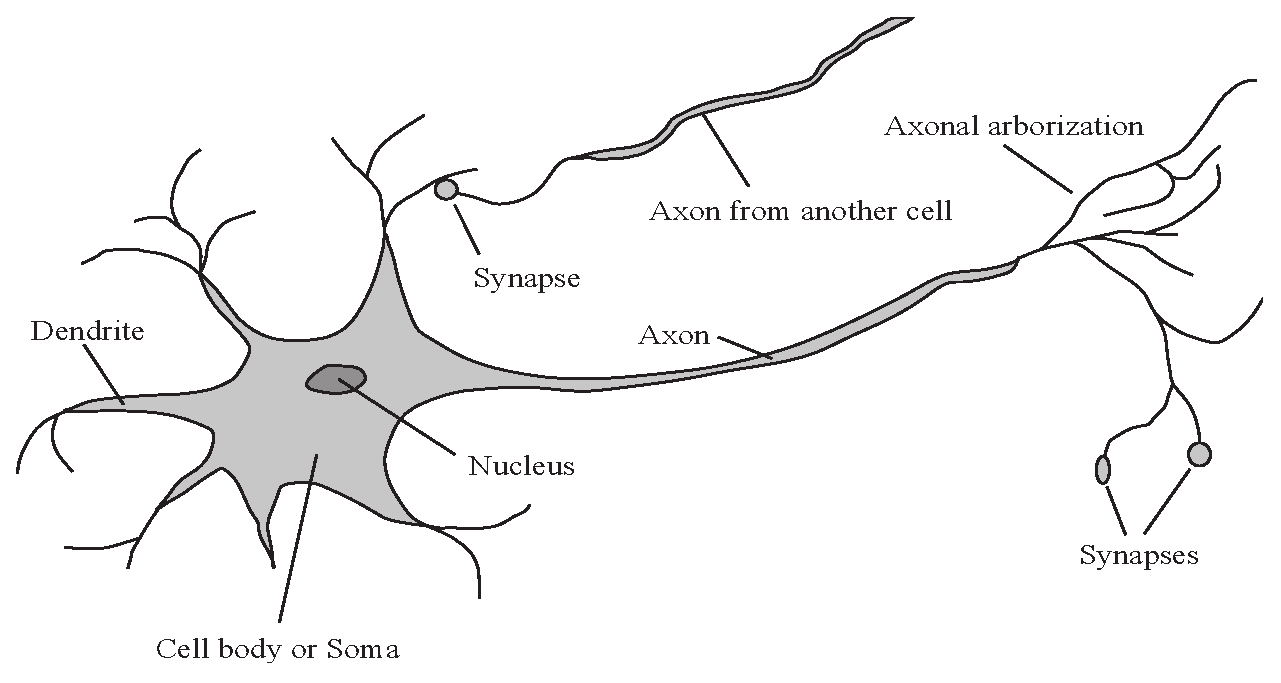
\includegraphics[width=0.95\textwidth]{ModellAvNeuronet.eps}
	\caption{A illustrative model of the neuron. The signal propagation goes from the left to the right in this figure;
			Synaptic integration at the dendrites, action potential through the axon and finally transmission throught the output synapses. 
			The aspects of the cell body is not immediately relevant to signal processing, and is not taken into account in the model used. }
	\label{figFigurAvNeuronet}
\end{figure}

% Gjennomgang, natt til 30juli. Her er eg no.
% TODO TODO TODO TODO TODO TODO TODO TODO TODO TODO TODO TODO TODO TODO TODO TODO TODO TODO TODO TODO TODO TODO TODO TODO TODO TODO TODO TODO TODO TODO TODO TODO TODO 

When the action potential reaches the ``axon terminal'', where the presynaptic membrane of the synapse lies, neurotransmitters are released into the synaptic cleft 
 	(se appendix \ref{appendixSecPresynapticSynapticPartOfTransmission} for a more complete discussion of the action potential and the presynaptic elements of synaptic transmission).
The neurotransmitters diffuse passively out in the synaptic cleft. Some come in contact with the postsynaptic receptors, and activates the receptor.
%The receptors that are relevant to this project is the ligand--gated receptor group.
%Describing the different known kinds of receptors will be outside the scope of this report. We will limit the description to one class of receptors, called ``ligand--gated receptors''.
Directly--gated receptors (also called ``ligand--gated channels'') open a channel when exposed to the right ligand (the right neurotransmittor), 
	causing an increase or decrease in the postsynaptic neurons depolarization\cite{PrinciplesOfNeuralScience4edKAP10}. .
%Ligand--gated receptors are direcly connected to ion channels in the membrane. Opening of these ion specific channels enables some ions to flow throught (depending on what kind of channel the receptor is connected to). 
%Depending on which ions are let through, the neuron is either depolarized (towards zero polarization, less than its resting potential) of hyberpolarized (getting a more negative membrane potential) by the transmission.
Whether the postsynaptic depolarization is increased or decreased by a synaptic transmission defines the synapse as being an excitatory or an inhibitory synapse\cite{PurvesNeuroscienceKAP05}.
%On the postsynapsic membrane in the synapse are different receptors for different neurotransmitters\cite{PrinciplesOfNeuralScience4edKAP10}. 
%The receptors are only activated by some neurotransmitters, and the change in postsynaptic postential varies with what ions the receptor channel is permeable to.

%Since depolarizing the neuron causes firing, the neurons potential is often referred to as the neurons depolarization in the litterature.



\subsection{The Axon and the Action Potential}
\label{ssecTheActionPotential}
In the membrane of the axon we have voltage--gated channels that open if the level of depolarization is more than some value. This value is called the ``firing threshold of the neuron''.
These channels will open and further depolarize the membrane. 
Through passive transmission of the electrical potential, the next voltage gated channels will open as a result of going above the gate threshold. %also go beyond the firing threshold.
This establishes the active aspect of action potential propagation, and results in a self carrying propagating through the axon.
%This establishes the self carrying signal of the axon, and results in an equal depolarization at the different axon terminals\cite{PrinciplesOfNeuralScience4edKAP09}.
An important result of this is that the presynaptic membrane at the synapses recieves an equal depolarization, independent of its location. 
The release of neurotransmitters is a result of this depolarization, and the action potential enshures an equal depolarization of the presynaptic membrane.
This gives that the transmission is dependent only on the synaptic connection, or ``the synaptic weight''\cite{PrinciplesOfNeuralScience4edKAP09}.
%
%This means that sufficient depolarization of the membrane of the axon opens voltage gated ion channels that will further depolarize the membrane. 
%Through passive transmission of the voltage, the signal is distributed to the next voltage gated channels.

%todo skriv mot slutten av paragraf:  The voltage gated channels will only be open for a small period of time.
%There are at multiple kinds of voltage gated channels. The sodium channel opens
For the action potential there are two important voltage--gated channels; The sodium channel and the potassium channel.
The $Na^{1+}$ channel opens faster than the $K^+$, and gives the rising phase of the action potential.
The rising phase of the action potential comes as a consequence of more positively charged $Na^{2+}$ ions outside the neuron causing a strong inward current after opening of the $Na^{2+}$ channels.
Voltage gated $Na^{2+}$ only stay open for about 1 ms before they close.
About the same time as the $Na^{2+}$ channels close, the $K^+$ channels open. 
Because there is a larger concentration of $K^+$ inside the cell, this will cause a more negative potential over the membrane. The neuron is repolarized.
%After some time delay, the $K^+$ channel opens, and at about the same time the $Na^{2+}$--channel close.
%We have more $K^+$ ions inside the cell, so increasing the permeability for $K^+$ will decrease the depolarization over the membrane, or ``repolarize'' the membrane.
%When both channels are closed again we are back at the resting potential of the neuron. %SITER: Bear s:91
After the action potential the membrane potential is ``reset''.
As the electrical potential spead passively to the next site with voltage--gated channels, 
	the refraction period of each voltage gated channel is an impotant mechanism to hinder the action potential from going ``the wrong way''\cite{NeuroscienceExploringTheBrain3edKAP4}\cite{PrinciplesOfNeuralScience4edKAP09}.

To recreate the ionic gradient, the ions are transported back by the sodium--potassiom pump.
As this is a mechanism that use a little time to reset the ionic gradients, we have a little period when the gates have to be closed.
This is the basis for the refraction period of the neuron, a small period of time where action potential cannot be initiated\cite{NeuroscienceExploringTheBrain3edKAP4}.

After firing an action potential, the neuron will also have a short period where it is impossible to exite the cell, called \emph{the absolute refraction period}\cite{PrinciplesOfNeuralScience4edKAP09}.. 
%The refraction period of a neuron usually lasts for a few milliseconds\cite{PrinciplesOfNeuralScience4edKAP09}.
%\cite Bear kap. 4  (s.91, nede) og Kandel kap.9 s 157 (nede)
%TODO TODO TODO TODO TODO TODO TODO TODO TODO TODO TODO TODO TODO TODO TODO TODO TODO TODO TODO TODO TODO TODO TODO TODO TODO TODO TODO TODO TODO TODO TODO TODO TODO TODO TODO TODO TODO TODO TODO TODO TODO TODO TODO TODO 
% Plan: finn referanse på dette, og så sei at eg har matematisk vist det å være sant.
In this project, the author has demonstated matematically that the refraction period is important for limiting the firing frequency of the neuron. 
The analysis is presented in section \ref{ssecValueOfAlpha}.
%In this project the author has formalized that the refraction period is important for limiting the firing frequency of the neuron. The analysis is presented in section \ref{ssecValueOfAlpha}.


%												"close to":  SKRIV OM
The axon is organized as a tree, with a trunk in close proximity to the soma of the neuron, called the axon hillock.
The branches of the ``axonic tree'' are called axon collaterals. 
The elements of the axon that is furthest from the axon hillock is called the axon terminal, and is where the output synapses are located.
%The axon ``ends'' in the axon terminal, where the presynaptic part of the synapse is located.
When the action potential reaches the synapse, a transmission is initialized by the opening of voltage gated $Ca^{2+}$ channels\cite{PrinciplesOfNeuralScience4edKAP10}.
%The signals transmitted in the axon is strictly directional, that is: the signal goes from the axon hillock (close to the neurons soma) to the axon terminals (where the synapses is). 

%ODO Skriv mindre, eller i det minstre mindre kraftige utsagn. Følgande er rett, men kanskje urelevant for denne oppgava?
%You also have modulatory synapses at the axon terminal, that does not contribute to the value of the neuron, only the amount of neurotransmitters released following the next incoming action potential. 
%The modulatory synapse is but an example of the complexity of the simplifications that are neccesary in order to make an artificial neural network.
%In addition we have different time delay for different synapses along the axon, diffuse modulatory systems it the brain with modulatory neurotransmittors, 
%different states as the neurons use the oxigene and nutritients available, etc.






\subsection{The synapse}
\label{ssecTheSynapse}
%\subsubsection{Synaptic Plasticity}
%When the action potential reaches the axon terminal, the size of the signal is thought to be the same as when it first was initialized at the axon hillock.
%This enshures that the distance the action potential has to travel does not affect the transmission at the synapses of the different axon terminals. \cite{NeuroscienceExploringTheBrain3edKAP4}.
Following an action potential, voltage gated $Ca^{2+}$ channels are opened and $Ca^{2+}$ enters the axon terminal.
This causes synaptic vesicles to merge with the presynaptic membrane, causing the content of the synaptic vesicles to be released into the synaptic cleft. %Cite Kandel kap.10
% Forrige to linjer (passer med siste forrige section) ELLER neste linje:
%When an action potential reaches the location of a particular synapse, the membrane potential will cause release of neurotransmittors from the axon terminal (the presynaptic neuron).
%-------------------------------------------------------------------------ordna til hit-------------------------------------------------------------------------------------------------------------------------------------------
The neurotransmitters from the synaptic vesicles diffuse into the synaptic cleft.
If a so--called ligand--gated channel at the postsynaptic membrane is exposed to these neurotransmitters, the channel opens and ions are let thought.
The result is either excitation or inhibition of the postsynaptic node's value, depending on the channel (which ions are let through).
The size of the transmission is based on presynaptic and postsynaptic mechanisms\cite{PurvesNeuroscienceKAP05}.
%The transmission is thought to be a funcion of presynaptic and postsynaptic mechanisms.

\begin{itemize}
	\item Presynaptically, different amount of neurotransmitters can be released from the axon terminal following an action potential.
	\item Postsynaptically, the amount of receptors varies between different synapses. The amount also varies with time. % This is one mechanism of synaptic plasticity.
\end{itemize}

The level of transmission is the background for what is modelled as the synaptic weight in artificial neural networks.
%These two sides of synaptic transmission are important when synaptic plasticity is considered. 
Patterns of long term synaptic plasticity is what is what is percieved as learning in the field of neuroscience \cite{NeuroscienceExploringTheBrain3edKAP25}.
A more comprehensive study of synaptic plasticity is outside the scope of this text, but it should be mentioned that the ion $Ca^{2+}$ is thought important in both presynaptic and postsynaptic plasticity.
The postsynaptic role of $Ca^{2+}$ is important for STDP, which is an important argument for ANN with the capability of calculating the spike time.
%This is important for STDP, which is an important argument for ANN with the capability to calculate the timing of the spike.
For the especially interrested, appendix \ref{appendixSynPlast} considers presynaptic and postsynaptic mechanisms behind synaptic transmission and synaptic platicity, with a special focus on the role of $Ca^{2+}$.








% //{ Kommentert ut.  Gave til meg selv når eg skal skrive masteren (liten gave, nesten ingenting)

% //{
%The conclution from the study about 

% % XX MED-noke-om: For now, it is enough to mention that the synaptic weight changes as a multifactorial function based on 
%For now, it is enough to mention that  $Ca^{2+}$ is important both presynaptically and postsynaptically for synaptic plasticity.
% % We will later make use of some of the 
% % XXX Bra, men passer det inn:
%When the action potential reaches the axon terminal, it will open voltage--gated $Ca^{2+}$ channels in the active zone of the terminal, and $Ca^{2+}$ enters the cytosol of the axon terminal of the presynaptic neuron\cite{PrinciplesOfNeuralScience4edKAP10}.












% The signal arriving at the presynaptic membrane is equal for all the synapses, the transmission is not. 
% The transmission varies as a function of many mechanisms. %xxx Dårlig setning!
% For the scope of this text, we will focus on the mechanisms within the neuron. 
% I will refer to the size of this transmission as the weight of the synapse. 
% % Dårlig skrevet, over her.

%In this report the convention used by Rolls and Treves in ``Neural Networks and Brain Functions'' will be used. 
%For any transmission through a synapse between neuron $j$ and neuron $i$, we define the synaptic strength $w_{ij}$. 
%Note that the first subscript refers to the recieving neuron and the last subscript to the presynaptic neuron (the signalling neuron) \cite{TrevesNeuralNetworks}.
%This convention will be used in this text. 







%This does not mean that the transmission for different synapses is the same. At each synapse the connection to the postsynaptic neuron is different. 
%There are many mechanisms behind this, but I will focus on the mechanisms within the neuron:
% //}

%\subsubsection{Presynaptic mechanisms behind synaptic plasticity}
% //{
%$Ca^{2+}$ causes release of neurotransmittors from the presynaptic axon terminal into the synaptic cleft\cite{PrinciplesOfNeuralScience4edKAP10}. 
%Long--term potentiation (LTP) causes a lasting change of the tranmission through the synapse.% On the shorter time scale we have short--time potentiation, called fascilitation and short--time depression (decrease of transmission) called 
%
%The amount of $Ca^{2+}$ inflow, and thus the amount of neurotransmitter release can be modulated by socalled axoaxonic synapses\cite{NeuroscienceExploringTheBrain3edKAP5}, synapses that is connected directly to the presynaptic axon terminal. 
%A transmission here will cause a small increase in the axon terminals amount of $Ca^{2+}$ and ``prime'' the synapse for a transmission. 
%Multiple incoming action potentials in fast succession will have the same effect on the following action potentials and causes what is called \emph{potentiation} (short term increase in synaptic weight)
%\cite{PrinciplesOfNeuralScience4edKAP14}. 
% %Variation of the $Ca^{2+}$ entering the presynaptic axon terminal, for example by ``priming'' the synapse for transmission by axon-synaptic synapses, is one potential mechanism for synaptic plasticity\cite{PrinciplesOfNeuralScience4edKAP14}.

% X XX Ta vekk mykje av "Presynaptic mechanisms behind synaptic plasticity" om eg ikkje bruker desse effektene i implementasjonen!
% //}


%\subsubsection{Postsynaptic mechanisms behind synaptic plasticity}
% //{
%Glutamate is the main excitatory neurotransmittor in the CNS\cite{PrinciplesOfAnatomyAndPhysiology12edKAP12}. %s. 448
%There are two main groups of ligand--gated glutamate receptors, the N-methyl D-aspartate (NMDA) receptors and the non-NMDA receptors. 
%The non-NMDA receptors mainly consists of the $\alpha$-amino-3-hydroxy-5-methyl-4-isoxazolepropionic acid (AMPA) receptor. %XXX SITER!
%
%Most non-NMDA receptors are permeable to ions that changes the postsynaptic potensial without having lasting changes on the synaptic strength.%efficiancy. 
%The NMDA receptor is permeable to $Ca^{2+}$, which is important for lasting changes of the synaptic strength. %uttrykket 'synaptic strength' har ikkje blitt definert enda. Gjør det lenger oppe. XXX DO IT!
%
%An other important difference between the NMDA-R and the AMPA-R is that NMDA receptors have an additional condition for opening of its ion channel. 
%In the NMDA receptor there is a $Mg^{2+}$ ion blocking the channel. 
%When the potential across the membrane is sufficiently depolarized, the $Mg^{2+}$ will float more freely and the block is removed from the NMDA receptor.
%$Ca^{2+}$ diffuses into the cell following an action potential\cite{PrinciplesOfNeuralScience4edKAP12}.
%
%Also on the postsynaptic part of the synapse $ca^{2+}$ has an important role in synaptic plasticity. 
%$Ca^{2+}$ activates production of more non-NMDA receptors for the postsynaptic membrane, resulting in LTP\cite{AMPARtrafficingArtikkel}.%\cite{PrinciplesOfNeuralScience4edKAP12}.
%
% %TODO Det under gjelder jo bare for kvifor vi får positiv vektendring. Skriv dette, eller finn ut forklaringa for negativ vektendring (LTD) som følge at STDP! XXX
%The NMDA-related synaptic plasticity is the background for what is called ``Spike Timing Dependent Plasticity'' (STDP) that will be important later in this text.
% % XXX ikkje "rest of this text." Det er ikkje viktig over alt. Noken plasser.. Kanskje "an important element in this text."?
% %Skriv om hebbian learning, ustabilitet  og at STDP kalles "stable hebbian learning". Sjå rapport i NEVR3004.
% %STDP has also been called ``stable hebbian learning''. This refers to the 

%\subsection{SKRIV OM STDP! Referer til forrige avsnitt}
% %TODO: sjå rapport NEVR3001, NEVR3003.
% %HER ELLER OVER. kjør \label{forklaringBakSTDP}
% //}

%\label{forklaringBakSTDP} %der forklaringa kommer...

%\subsection{Skriv om Dale's  principle}
%At eit neuron kan sleppe bare en neurotransmittor (eller to, fleire). Desse kan gi ulik virkning på ulike receptore, men i utgangspkt. kan man sei at eit neuron enten er excitatory eller inhibitory. 
%Men dette er også feil. Drøft fram og tilbake.. Skriv konklusjonen (til korleis eg gjør det i min implementasjon) i section{implementation}.


% %Because of the boolean nature of the action potential, the transmission of the action potential to the next neuron is desided by the strength of the synaptic connection.

% %The most studied neurotransmittor is glutamate. In most neurons glutamate is an excitatory 

% %Skriv om STDP (glutamate), om bakgrunnen for STDP: NMDA med mg²⁺ blokk, voltage dependent i tillegg til at utsida må være eksponert for glutamat, Ca²⁺ inflow fører til AMPA-syntese => synaptisk plastisitet! 


%\subsection{nettverket}
% - Med booleanske signal: korleis kan signalet inneholde så mykje informasjon?
% 		- skriv om inter-spike period. Og kanskje om ANN-flyttals variablene som output fra neurona..
% //}

\newpage
% Her skal eg skrive om den nye modellen. Kva er \kappa, kva representerer denne, tid går mot uendelig.. osv.

% Disposisjon:
% 
% 1) kva gir depol. for ein neuron. Kva gir input, kva gir lekkasje?
% 2) utledning av depol.-ligning
% 
% 	TODO Lag frampeik om at "dette kan brukes til ANN", eller tilsvarende.
%

\section{Mathematical modelling of the biological neuron} 
\label{secMatematiskModelleringAvBioNeuron}

%Når eg skriver om:
% Fokuser mest på at value, dvs. depol. til neuronet er kva som er viktig i forhold til fyring av AP. Difor bør vi prøve å modellere dette.
% Ikkje tenk på Nernst, her. Det kommer i neste avsnitt.

Mathematical modelling of the neuron helps understand the neuron, and the mechansims behind how the neuron works.
A good model of the neuron will also give us a guide when simulating the system.

In the neuron, the value of each node is given by the electrochemical potential over the cell membrane. 
The neuron will fire an action potential if the value goes over the firing threhold. This makes the value of the neuron an important aspect of neuronal signal processing.
When a neuron recieves a synaptic transmission, ligand--gated channels are opened, and the potential of the neuron is changed as a function of the time the channel is open, and the electrochemical driving force for the charged molechules.
One part of the driving force is given by the electrical potential over the membrane. % XXX vent med dette : When ions are allowed to flow through a channel, the amount that will flow is given
The electrical potential can be seen as a potential field for charged particles.
An other element of the driving force is the distribution of the indivitual ions. Ions are transmitted across the membrane by passive diffusion. 
This meens that the indiviual ions are pushed down its concentration gradient.
If we combine these two effects we get a simplified system of the neuron.
%TODO REFERER: \ref{NeuroscienceExploringTheBrain3edKAP3}
%TODO TODO Skriv om! Bare rot!

% TODO Slett det under. Skriv alt heilt om!
In the biological neuron, the value of the node is governed by many factors. 
The individual ion's equilibrium potential can be calculated by the Nernst equation (eq. \ref{eqNernstEquation}).
%TODO Vent med dette:    For the artificial neuron the value corresponds to the membrane potential of the biological neuron.


The membrane potential of the biological neuron is given by the distribution of electrically charged particles and molecules over the  membrane.
The electrical potential is an impoirtant part of the driving force for changing the value of the node.
From this we can later talk about the differential equation of the nodes value.
%These are two of the mechanisms that gives the 
%The electrical driving force is not the only one, and the value of the node at equilibrium is given by the sum of all these driving forces.
%An important equation in this respect is the Nernst equation.


% TODO TODO TODO TODO TODO TODO TODO TODO TODO TODO TODO TODO TODO TODO TODO TODO TODO TODO TODO TODO TODO TODO TODO TODO TODO TODO TODO TODO TODO TODO TODO TODO TODO 
% Skriv også at simulering er basert på modellering, og at bedre modellering gir oss inspirasjon til nye typer simuleringer. (sikt veldig til meg, uten å sei det..)
% Det fører også til bedre simuleringer?



\subsection{The equilibrium potential}
% TODO TODO Skriv også om lekkasje! Fra ANN.tex refererer eg hit når eg snakker om lekkasje. XXX Hugs å skrive om lekkasje her!
% Sjå ANN.tex: Snakker om LIF-neuron. Skriv om LIF-neuron når eg skriver om lekkasjen!
\label{ssecTheEquilibriumPotential}
%TODO Er det her eg skal skrive om LIF-neuron (leaky integration)?
In the biological neuron, the reversal potential for the different ions is can be calculated by the Nernst equation. 
The reversal potential is the electrical potential where the respective ion flow will be revesed (flow the oposite direction) if an ion channel is opened.
This also involves that at the reversal potential, we get no ionic current following a channel opening. 
This is due to a balance between the driving force provided by the concentration gradient of the ion and the electrical driving force.
The reversal potential is also called the equilibrium potential.
%The reversal potential is the potential where opening of the ions channel causes no net current flow through the membrane.

% XXX Skrive inn nernst-equation? Referer kapittel 3 i Bear. (s 65)
\begin{equation}
	\label{eqNernstEquation}
 	E_{ion} = \frac{C}{z} log\frac{[ion]_o}{[ion]_i}
\end{equation}
Where $E_{ion}$ is the equilibrium potential for the ion, C is a constant (for some temperature), z is the charge of the ion and $[ion_i]$,$[ion_o]$ gives the number of ions on the inside and outside of the membrane
\cite{NeuroscienceExploringTheBrain3edKAP3}.

For a neuron permeable to a single ion, the equilibrium potential will be the same as this ion's equilibrium potential. %ref kandel kap 7. s129
For systems where permeability of multiple ions are involved, the equations for each ion becomes a sum of electrical driving force and chemical driving force multiplied with membrane conductance for the ion
\cite{PrinciplesOfNeuralScience4edKAP07}.
%skrive om at dette gir oss at for en komplett simulering av dette, trenger vi en variabel som holder orden på kvart ion.
A good simulation of the system therefore should have one variable for each of the electrically charged particles and molechules.
There are many important ions and also a couple of protheins and neurotransmittors that are electrically charged, so this will introduce a large computational load in the simulation.
%Many, if not all of the previous implementations I have seen have a simplified structure for the node's value, by having one activation value; The electrical potential.
To my knowledge, no implementation of SANN with a pragmatic use (i.e. used in technology) uses multiple ions to find the depolarization of the nodes in the simulation.
These implementations use the electrical potential as the value for each node. This will also be the focus of the remaining part of the modelling section.
%It is unknown wheter this removes any important aspects of the neuron.

% Todo: Skriv om neste linja!
At rest, the membrane is permeable to some ions, and to prevent the ion reaching (and staying) at the neurons equilibrium potential, there are active pumps maintaining a different potential. 
%
In the postsynaptic membrane of some synapses there is so--called \emph{ligand--gated ion channels}, channels that are activated by exposing the activating neurotransmittor\cite{NeuroscienceExploringTheBrain3edKAP5}.
The channel will be open for a small time period, causing a flow of the ions that are let throught the channel, giving an altered postsynaptic potential. 
Excitatory synapses increase the postsynaptic node's value. This is called an Excitatory PostSysnaptic Potential --- E-PSP \ref{PrinciplesOfNeuralScience4edKAP07}.

Other ligand--gated channels have other channels that will decrease the value of the neuron.
%Inhibitory synapses have other channels that causes an inhibition of the postsynaptic neuron. 
Because this inhibits the neuron in respect to firing an action potential, this is called inhibitory synapses, and the postsynaptic effect of a transmission is called Inhibitory PostSynaptic Potential (I--PSP).
%This involves decreasing the postsynaptic neurons value. This is called an Inhibitory PostSynaptic Potential (I-PSP).
%XXX ref kap 7. kandel.
Because of time limitations, modelling of the time delay and size of each transmission has not been evaluated in this project.
An other aspect that will be for further research, is modelling and implementation of synaptic plasticity. 
This is one important reason behind using artificial neural networks in technology, and the reason behind developing the spiking variant of ANN.
Synaptic plasticity will hopefully be modelled and implemented in a later project.
%This project is about the comparison between 

%Opening of a membrane channel will change the permeability of the membrane to some ions (depending on the channel), and the ion pumps will not be able to maintain the potential different from the equilibrium potential. 
%This causes the potential of the neuron to change accordingly, and is the basis of exitatory and inhibitory postsynaptic potentials (E-PSP/I-PSP)\cite{PrinciplesOfNeuralScience4edKAP07}.
%X XX ref kap 7. kandel. s. 131




Some of the aspects in the theory of the electrical potential for the neuron was introduced to show that the simulated system is a complex one, even at the level of the individual node. %Videre har vi også at proteiner kan ha ladning.
For each node we have a complex system with a continously changing driving force and membrane conductance for each ion. 
For artificial neurons used in an ANN most of these aspects can be simplified without affecting the result much. 
Because the primary focus for this implementation is the use of the neural simulator in technology, the efficiancy of the implementation is crucial. 
We therefore have a single variable giving the membrane potential as the activity variable in this implementation. 
The extra computational load introduced by multible activity variables is not worth is for simulators with a pragmatic focus. %Kva meines med pragmatic focus? Skriv dette..
%TODO SJå over avsnittet og få bedre flyt!
%In addition this is the VANLIGE INNEN SANN.

%It is also important to know about the complex structure of neural signal processing


%Rensa opp litt til hit. *********** fortsett rensing herifra. ****************


%skriv om neste:
%The reason for introducing the background information about the neuron is  %TODO SKRIV OM: Skriv at det er viktig for å forstå simulatoren min(meir om dette seinere). XXX Ta vekk denne itemize(?):
%\begin{itemize}
%	\item to introduce the ide of different states for the neurons membrane. Each with its own equilibrium potential.
%	\item to introduce an important consept for the neuron that will be important for ANN as well, $V_{r}$.
%	\item to describe the complexity of the system. For a complete simulation of a neuron, each ions distribution across the membrane may need to be simulated as a dynamical system.
%	\item to give the background for the system to be modelled as a leaky integrator. The neurons value ``leaks'' toward the equilibrium potential.
%\end{itemize}














\subsection{------------SKREVET OM TIL HIT.----------}





$V_{r}$ will be used as the resting membranes potential. For biological neurons this can be calculated by the Goldman equation\cite{PrinciplesOfNeuralScience4edKAP07}. 
For our use if will be enough to know the extistance of the equilibrium potential for a membrane at rest,
in addition to define a resting membrane potential for the implementation of the artificial neuron.

%For multi--ion systems modelling the system becomes more complicated, but for our use it is enough to know that there is a resting membrane potential that is a function of


% TODO Minimaliser reperering av det er nettop har sagt.. XXX

%It is important however to know that there is such an equilibrium potential, given by the sum off all the contributions (from the individual ions).

Because of the active pumps, different states with different permeability do the different ions will give different membrane potential because of different factors for each part of the ion differential equation. 
The membrane at rest, that is with no open ion channels, gives the resting membrane potential, $V_r$. 

In the case of synaptic input to a neuron, the postsynaptic membrane will open ligand gated channels (se section \ref{ssecTheNeuron}). 
Both for exitatory and inhibitory input this will push the neurons value and could be seen as an external force in the system.
%For our use, we set this external force to be a constant.
Whether this external driving force can be percieved as a constant or is a more complicated dynamical system is as everything else in the nature; complicated. %Skriv slutten analeis.
The neuron has NMDA channels that are more permeable to both the normal ions in addition to $Ca^{2+}$. Since the NMDA-R is voltage dependent, this causes the glutamatic transmission to be a function of the postsynaptic potential.

%For E input. Kva skjer. Sjå på som eksternt pådrag. 
As this is a mechanism that is little described in articles in neuroscience and to my knowledge not used in ANNs, I will not use voltage dependent exitatory ion channels in my two implementations of ANN. 
%Skriv at dette uansett ikkje har noko innverkning på resultatet? Eller blir dette også dumt i forhold til relevansen til denne linja i teksten?
For my implementations the external driving force on the membrane potential will in other words be a constant.

%Skriv om lekkasje. Forbered på neste seksjon.
%When the potential over the membrane does not equal this equilibrium potential, the system will be driven toward this equilibrium. %(without any external input).

%In the case of neural networks, this is called a 'leaky integrate-and-fire' (LIF) model.

%TODO Poengter at dette er mitt arbeid:
\subsection{The differential equation for neurons depolarization} % (gjør om chap til sec. ,no. Skal denne bli subsubsection?
The equation for the potential can be stated as a first order differential equation:
\begin{equation}
	\dot{v}(t) = \dot{v}_{in}(t) - \dot{v}_{out}(t) %, \qquad i = \text{ neural input } %% XXX Endra \dot{v}_{in}(I) til  \dot{v}_{in}(t). XXX
	% skriv også at det er \dot{v}_{out]}(t, v(t)) ---avhengig av v(t) også!
\end{equation}
Where $\dot{v}_{in}(t)$ gives the effect of synaptic input to the neuron% XXX KVA er PÅDRAG på engelsk?
	, and $\dot{v}_{out}(t)$ represents the ``leakage'' of the neurons value.



% TODO Ikkje del opp i underavsnitt: Skriv heller "Element for diffligninga", eller noke, og få med begge her.
% Men det eg heller kan ha med som underavsnitt er "forkrav for ligningene" eller "utgangspkt" eller "antagelser for ligningene"...
\subsubsection{The input}
The input, represented by $\dot{v}_{in}(i)$ in the above equation, is a function of the neurons exitatory and inbibitory input. 
The neurons input waries with time, but for now we look at the variable $I$ as a constant in respect to time.
%One method for a varying degree of input will be introduced in section \ref{ssecVariableInputBetweenSpikes}.
Later, in section \ref{ssecVariableInputBetweenSpikes}, the method will be expanded to account for a varying degree of input. % (section \ref{ssecVariableInputBetweenSpikes}).

\begin{equation}
	\dot{v}_{in}(t) = I
\end{equation}
%$I$ is the effect of the input to the neuron (sum of exitatory and inhibitory input).
$I$ represents the effect of the synaptic input to the neuron at time $t$, the sum of the effect of exitatory and inhibitory input to the neuron.

%skriv også at v_in(i) er i virkeligheita eit dynamisk forløp, men for ANN kan vi forenkle, og sjå på denne som konstant.


\subsubsection{The ``leakage''}
%TODO Finn referanse for neste påstand!
The neuron is often modelled as a leaky integrator. The ``leakage'' is dependent on the polarization over the membrane. 

For biological neurons, the leakage is given as a function of the difference between the membrane potential and the resting membrane potential $V_r$. 
If we define the resting membrane potential for our artificial neuron to be zero, the leakage will vary propotionally to its potential $v(t)$.

%For artificial neurons, we can set this equilibrium potential to zero %for letthetens skuld. Kva blir dette på engelsk?
\begin{equation}
	\dot{v}_{out}(t) = \alpha v(t)
\end{equation}

In a biological neuron, the propotionallity constant, $\alpha$ is given by the distribution of different ion channels active at rest, the extracellular ionic environment compared to the intracellular level of the different ions, etc.
For our basic ANN this will be cept constant. For more advanced versions of this simulator, $\alpha$ could vary as a function of the intracellular ion--levels. 
In addition we have that the extracellular ionic environment is to large extent maintained by glial cells.
%In the CNS you have so--called astricytic domains governed by astrocytes (a certain kind of glial cell). In this domain the 
% BRIFEKUNNSKAP:XXX :  In the CNS you also have socalled astrocytic domains, where the support--cells for the neurons have domains. Inside this domain one astrocyte is 


\subsection{The depolarization equation}%equation for the neurons value}
This gives us the differential equation 
\begin{equation}
	\dot{v}(t) = \dot{v}_{in}(I) - \dot{v}_{out}(t) = I - \alpha v(t)
\end{equation}

Laplace transformation gives
% XXX Legg utledning av uttrykk i appendix! 		Her skal bare stå: V(s) = ...
\begin{equation}
	\begin{split}
		sV(s)-v_0 		&= \frac{I}{s} - \alpha V(s) 			\qquad, \; \qquad v_0 = v(t_0) 				\\
		(s+\alpha)V(s) 	&= \frac{I}{s} + v_0 														\\
		V(s) 			&= \frac{1}{s+\alpha}\left( \frac{I}{s} + v_0 \right)
	\end{split}
\end{equation}

And 
% XXX Legg utledning av uttrykk i appendix! 		Her skal bare stå: V(t) = ...  XXX type: bare siste linja i den kompilerte DVI'en
\begin{equation}
	\begin{split}
		v(t)  	&= 		\mathscr{L}^{-1}\bigg\{ V(s) \bigg\}  									\\
		 		&=		\frac{I}{\alpha} - \frac{I}{\alpha} e^{-\alpha t} + v_0 e^{-\alpha t} 	\\
				&= 		\kappa \left( 1 - e^{-\alpha t} \right) + v_0 e^{-\alpha t} 	\quad,\; \kappa = \frac{I}{\alpha} 
		\label{eqVerdiligninga}
	\end{split}
\end{equation}

The diversity of neurons makes it unrealistic to generalize over all neurons, and say to what the value is reset to.
For our artificial neuron we can define 
%Generalization for all neurons is unrealistic due to the divesity of neurons, but for our synthetic neurons we can define
that the neuron is reset to what corresponds to the equilibrium potential at rest, $V_r = 0$ after firing an AP.
%In the simulated neurons this means that after firing, the neuron is reset to $v_0=0$ after firing. 

The action potential is a discontinuity in the othervise continous system. The continous equation is only valid between action potentials (within one period).
%If we reset every aspect of the equation to be reset after firing, the equation can be used for the discontinous system. 
To use \eqref{eqVerdiligninga} for the whole time range, we define $t = t_{abs}-t_f$, where $t_{abs}$ is the absolute time and $t_f$ is the time of the last action potential. 
In this way $t$ represents the time since the start of the current period.

%If we define a time window as the time interval between time of reset (after firing) to next firing, we can define time $t$ as time after start of time window. This defines the time of reset as $t=0$.
%We define the time of reset as $t=0$.


%Equation \eqref{eqVerdiligninga} describes a continous nonlinear system. 
%In the neuron we have that if the neurons value goes above some threshold the neuron will fire an action potential, and the value is reset. This introduces yet another nonlinearity: 
%The action potential.

\subsection{The Action Potential}
The action potential, a ``spike'', and the period between action potentials, the interspike period, is the basis of the computational capabilities of the neuron.
When the value of the neuron excedes the firing threshold an action potential is initialized.
This causes transmission at all the output synapses of the neuron, and resetting the value of the neuron to $V_r$. % = 0. Skrive at det er lik null. Gjør likningene under rett..

We get that the neuron fires at time $t^*$:
\begin{equation}
	\begin{split}
			v(t^*) 					 							&= \tau \qquad 										\\	%,\qquad\qquad\tau = \text{firing threshold} 	\\
			\kappa (1-e^{-\alpha t^*}) + v_0 e^{-\alpha t})		&= \tau 											\\
	%		(v_0-\kappa)e^{-\alpha t^*}							&= \tau-\kappa 										\\
			\ln \left(e^{-\alpha t^*}\right) 					&= \frac{\kappa - \tau}{\kappa - v_0} 					\\
			t^*													&= -\alpha^{-1} \, \ln \left( \frac{\kappa - \tau}{\kappa - v_0} \right) 					
	\end{split}
	\label{eqTidTilFyringVedEndraKappa}
\end{equation}

Where $\tau$ is the firing threshold of the neuron. 
%XXX TODO Neste linjene er litt feil. Dette beskrive oppladninga av depol., m.a.o. ikkje heile p_isi(K). Bare p_charge,isi(K). Skriv dette. 
% ( Skriv at i tillegg får vi den såkalla "refraction time" errer eit AP. Dette må legges til for å få heile perioden.
If we define $p_d(\kappa)$ as the depolarizing phase of the inter--spike interval, for constant inter--spike $\kappa$ we get $v_0 = 0$, and the depolarization phase of the period is given by
\begin{equation}
	p_d(\kappa) = -\alpha^{-1} \, \ln(\frac{\kappa - \tau}{\kappa})
	\label{eqPeriodeligningForKonstIntraPeriodKAPPA}
\end{equation}

Equation \eqref{eqTidTilFyringVedEndraKappa} can also be used to calculate the time until firing for a given $\kappa$ and start value $v_0$
\begin{equation}
%	\begin{split}
	p_{r}(\kappa, v_0) 	\;= t^* + t_r 
						\quad= -\alpha^{-1} \, \ln \left( \frac{\kappa - \tau}{\kappa - v_0} \right) + t_r
%	\end{split}
	\label{eqRemainderOfPeriod}
\end{equation}
Here $p_r(\kappa, v_0)$ represents the remainder of the current inter--spike period and $t_r$ the absolute refraction period. % TODO XXX Skrive om dette? :  To see the refration time as a constant is a simplification.
The refraction period is more complex than so, but for our simple model we use this model of the refraction period.

It is impotant to remember that equation \eqref{eqPeriodeligningForKonstIntraPeriodKAPPA} and \eqref{eqRemainderOfPeriod} is based on a constant $\kappa$ during the whole period. 
% Det er meir komplisert enn det som står på neste linje. (gjør det litt større).
If $\kappa$ varies during the interspike period, the firing time will also change. %More on this in the next section.

%If $\kappa$ varies during the interspike period, $t^*$ from equation \eqref{eqTidTilFyringVedEndraKappa} is an estimate of the remainting time until firing. This estimate is updated every time $\kappa$ is.

%TODO Lag ei ligning for heile perioden også? Dette er bra å referere til!



\subsection{Variable input between spikes}
% TODO Skriv heilt om!
\label{ssecVariableInputBetweenSpikes}
Equation \eqref{eqPeriodeligningForKonstIntraPeriodKAPPA} is based on a constant $\kappa$ during the inter--spike period.
% TODO Skriv om neste poeng: kom inn på ideen / beskriv ideen om "time window".
%If we use this equation as the activation function of the node, we still can find the timing of the nodes action potential. STEMMER BARE DERSOM  if $\kappa$ is kept constant during the time interval.

%If $\kappa$ needs to be constant during the whole period, we get a large time lag for the system, so we need to devise a scheme for avoiding this.

If we allow the activation level of the node to change during the inter--spike period of the neuron, we cannot use \eqref{eqVerdiligninga} and \eqref{eqTidTilFyringVedEndraKappa} directly.
																			%the equations from the previous section.
To solve this problem, the concept of a ``time window'' is introduced. A time window is defined as the smallest of [a time interval where the activation level of the node is constant] or [the remainder of the interspike period].
%Within each time window both \eqref{eqVerdiligninga} and \eqref{eqRemainderOfPeriod} is therefore valid. % .. kan bli brukt.
Both equation \eqref{eqVerdiligninga} and \eqref{eqRemainderOfPeriod} is therefore valid within a time window.

\begin{figure}[hbt!p]
	\centering
	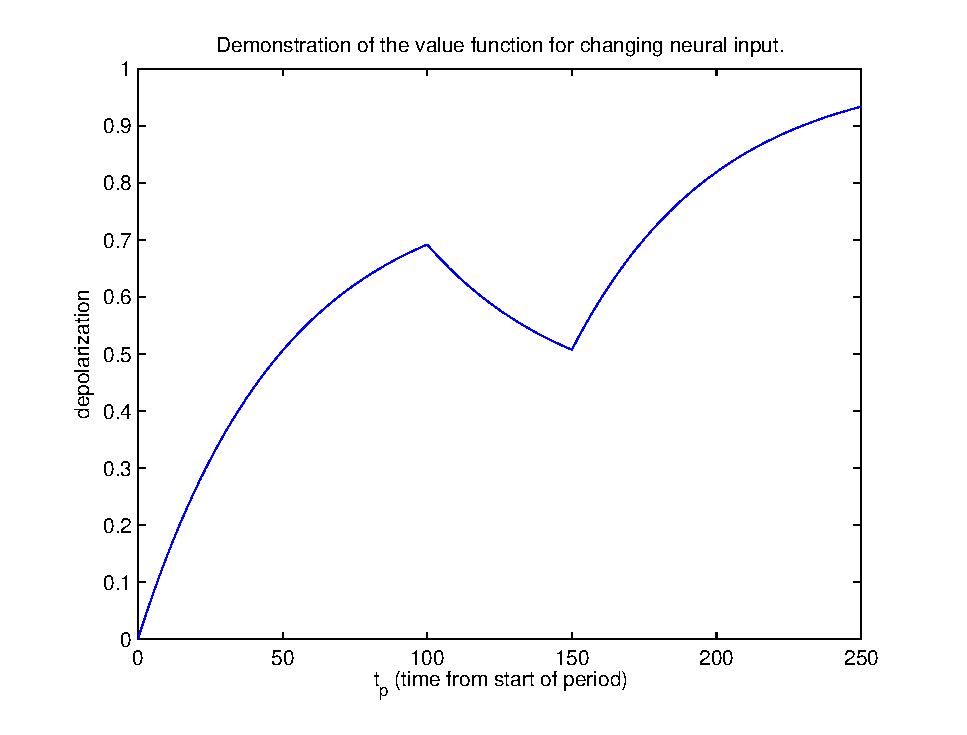
\includegraphics[width=0.95\textwidth]{demonstrasjonAvUlikeKappaforVerdifunksjonen.eps}
	\caption{$v(t)$ for changing $\kappa$. $\kappa_0=0.7$. At time $t_p=100$ $\kappa$ changes to $\kappa_1=0.5$. At time $t_p=150$ the neurons imput increases, and $\kappa$ becomes $\kappa_2=1$. See eq.\eqref{eqVerdiligninga}.}
	\label{figVerdifunksjonen}
\end{figure}

When $\kappa$ is changed, the initial value of the next time window, $v_0$, can be calculated from \eqref{eqVerdiligninga}. 
We can now use \eqref{eqTidTilFyringVedEndraKappa} to find the new estimate for the firing time of the node.
I use the word estimate because we can not know when $\kappa$ will change.
If $\kappa$ is changed before the estimated firing time, the firing time will be affected. 
%XXX if this is before the estimated firing time, the estimate of the next task time will change accordingly.  %If $\kappa$ is changed, the estimate changes.
%-> da er det "but an estimate of firing time.."

%Equation \eqref{eqTidTilFyringVedEndraKappa} gives us the time of firing for a situation where the initial value of the node can be different from zero.
%Also this equation is based on a constant $\kappa$.





%The equations can also be used as the non--linear activation function for a fANN. This activation function is based on a mechanistic model of the biological neuron.
%The activity can be read out of eq. \eqref{eqPeriodeligningForKonstIntraPeriodKAPPA} as the frequency $f(t) = \frac{1}{p(\kappa)}$
%
%If we let the activity level vary between spikes, the model will give as accurate timing as ``Spiking Artificial Neural Network''(SANN). We will discuss different aspects of artificial neural networks later. %XXX Ref?
%The model is based on fundamentally different equations than the model for SANN. 
%If this new model is as effective or more effective than SANN this project will be a contribution because we calculated the firing time in a new way.
%%Ta vekk siste, forrige linje?

%An other aspect with this new model is that it lies between the two prior models of ANN, and can easily communicate with both.

% If we allow the input and activity of each neuron to vary between spikes, the model approaches the model for the biological neuron.
% When $\kappa$ is updated, a new time window starts. 
% $v_0$ from \eqref{eqVerdiligninga} now represents the value at the start of the time window ( $v_0 = v(t=0)$ ). 
% This value is equal to the value $v(t)$ at the time of change of $\kappa$ from the previous time window(se fig. \ref{figVerdifunksjonen}).
% This is equal to the value of the neuron at the time of variation of $\kappa$ (the value at the end of the previous time window).

In fig. \ref{figVerdifunksjonen}, $v(t)$ is simulated for three different time windows. At time $t_p=100$, $\kappa$ changes from $\kappa_0=0.7$ to $\kappa_1=0.5$. At time $t_p=150$, $\kappa$ becomes $\kappa_2=1$. 
The simulation implies that the value function is a continous function that converges toward the neurons final value, $\kappa$, also when $\kappa$ varies.


With this new use of eq. \eqref{eqVerdiligninga}, we can calculate the remaining part of the neurons period after $\kappa$ changes value. 
The remaining time of the period is given by equation \eqref{eqTidTilFyringVedEndraKappa}, given constant $\kappa$. 
If this is updated each time $\kappa$ varies, we get an estimate of the remaining time based on the present $\kappa$.

%Skrive at dette plottet IKKJE er fra kjøring av programmet?




%TODO Finn eit bedre navn på denne subsubsection.
\subsection{The constants in the depolarization equation}
%\subsection{Redying the equation for use in ANN}
%TODO Skriv at denne ligninga kan brukes direkte for å lage en heilt ny modell for "spiking ANN" (ANN med information om 'spike-time').
% 	Om dette skal gjøres, må modellen tilpasses. Blabla, dette gjøres her. Eller noke.. Kanskje ikkje.
\label{ssecValueOfAlpha}

%TODO TODO TODO TODO TODO TODO 
% Skriv om 'value of alpha'! 	TODO TODO TODO TODO TODO TODO TODO 
%TODO TODO TODO TODO TODO TODO 

%XXX Veit ikkje om dette er relevant!

The inter--spike interval for a neuron consists of two phases. 
The absolute refraction period and the depolarizing phase (se sec. \ref{ssecTheActionPotential}).

Equation \eqref{eqPeriodeligningForKonstIntraPeriodKAPPA} describes the depolarizing phase of the neuron. % , $p_d(\kappa)$.
The equation for the whole inter--spike interval is given by
\begin{equation}
	p_{isi}(\kappa) = p_d(\kappa) + t_r
	\label{eqHeilePerioden}
\end{equation}

Where $t_r$ is the absolute refraction period of the neuron. % , and $p_d(\kappa)$ is given in \eqref{eqPeriodeligningForKonstIntraPeriodKAPPA}.
If we consider the firing frequency of the neuron, $f(\kappa) = p_{isi}^{-1}(\kappa)$ we can se that the asymptote is given by
\begin{equation}
	\begin{split}
		\lim_{\kappa->\infty}{ f(\kappa)} &= \lim_{\kappa->\inf}\left( \frac{-\alpha}{\ln \left( \frac{\kappa - \tau}{\kappa} \right) - \alpha t_r} \right)   \qquad = \frac{1}{t_r} \\ 
		%\lim_{\kappa->\infty}{ f(\kappa)} &= \frac{1}{t_r}
	\end{split}
\end{equation}

%Using l'Hôpital's rule %INNI ln(-) funksjonen. TODO Viktig å få med dette i denne setninga!
%and get %sjå wolframalpha.com ...
%\begin{equation}
%	\label{eqFrekvensLlim}
%	\lim_{\kappa->\infty}{ f(\kappa}) = \frac{1}{t_r}
%\end{equation}



We can see from this analysis that the refraction period of the neuron is fundamental for restricting the neurons output frequency (se fig. \ref{figFrekvensMedOgUtenRefractionPeriod}).
For biological neurons, the maximum firing frequency is about 1000 Hz \cite{NeuroscienceExploringTheBrain3edKAP4}. %s 79
\begin{equation}
	\lim_{\kappa->\infty}{ f(\kappa}) \approx 1000 \, \text{Hz}
\end{equation}
%If we define the maximum firing frequency to be 1000, equation \ref{eqFrekvensLlim} gives us the absolute refraction period as
We define the maximum firing frequency for the artificial neuron to be 1000 Hz. From equation \ref{eqFrekvensLlim} we get the absolute refraction period as
\begin{equation}
	t_r = \frac{1}{1000 \text{Hz}} = 1 \, \text{m}s %= 0.001 s = 
\end{equation}

%TODO Skriv at dette er en kjendt størrelse i neuroscience (finn, referer), og er en indikasjon på rettheten til lingningene (?)
% 		Kanskje også skrive litt om at dette er "absolute refraction period". Det er også en mild refraction period etter dette (finn,referer). Dette kan implementeres ved 2ms refraction period for auronet. 
% 		TODO TODO Sjekk andre linja her, og gjør en bestemmelse i forhold til mine ANN. (1 eller 2 ms refraction period?).
If we define the time step of the simulation to be 1 m$s$, the refraction period will be one time step in the simulation.
With a time step of 1 m$s$, the absolute refraction period (the time interval where it is impossible to exite the neuron) can be set to one time step. 
For SANN nodes, this means that the node will not change its value for the duration of the next time step. 
For $\kappa$ANN this can be implemented more effective by incrementing the estimated firing time by one time iteration. 
%TODO fullfør!


% Plott av frekvens med, og uten refraction period:
\begin{figure}[bhtp]
	\label{figFrekvensMedOgUtenRefractionPeriod}
	\begin{center}
		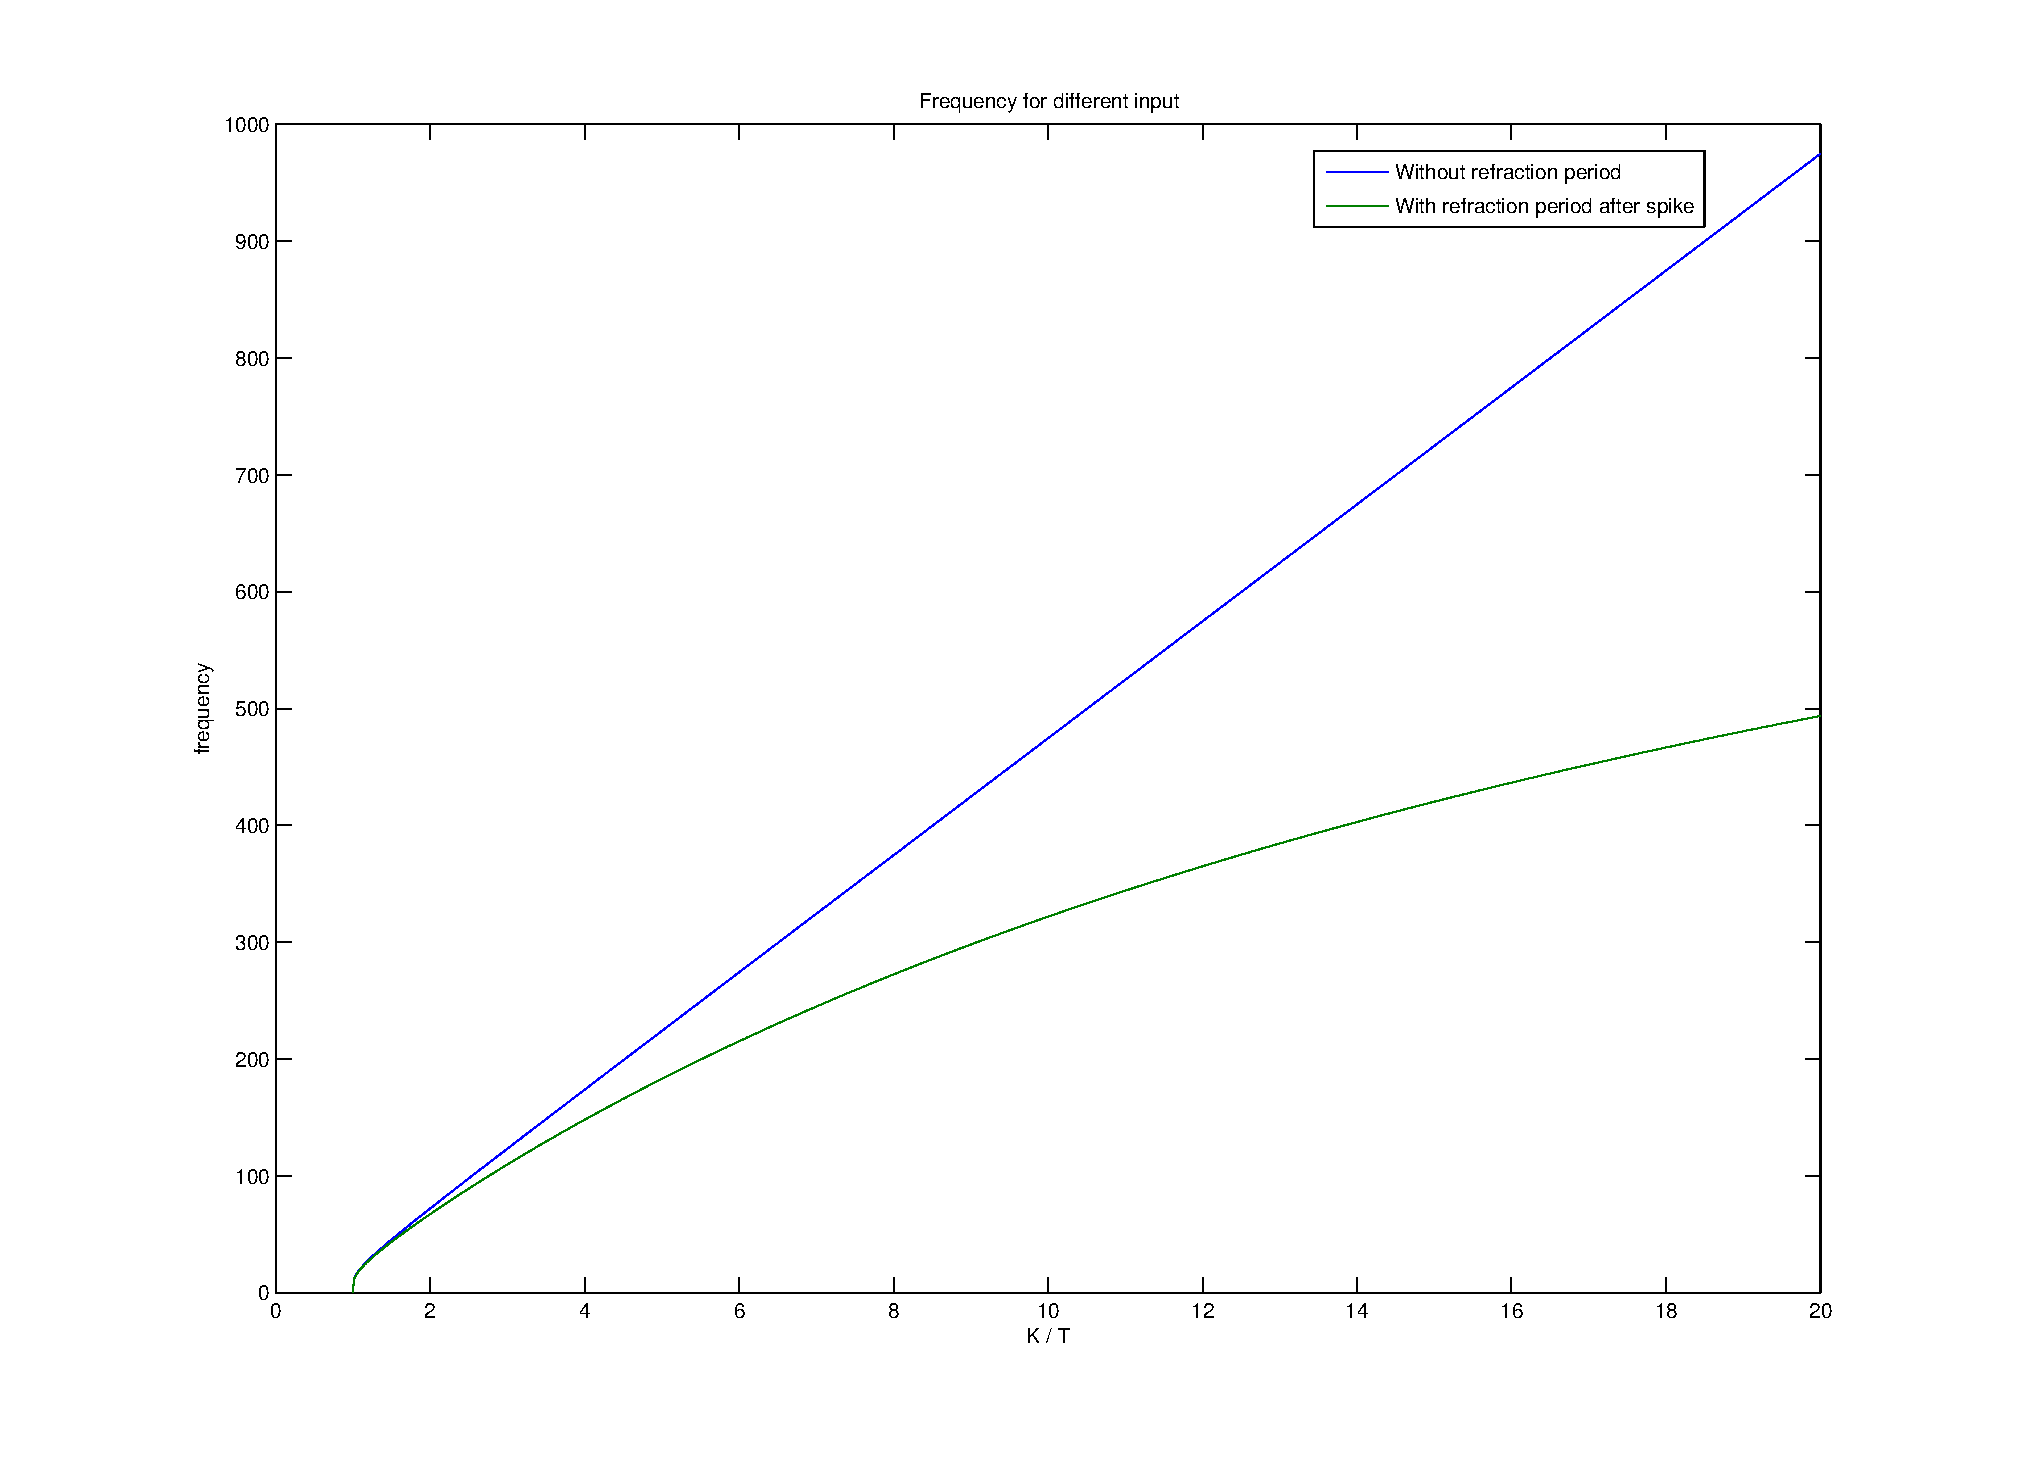
\includegraphics[width=0.95\textwidth]{frekvensPlotRefractionPeriod.eps}
	\end{center}
	\caption{Frequency for a neuron for different values of input. With and without refraction period}
\end{figure}



%TODO Skriv meir om kva de ulike variablane betyr. Kva er \kappa! kva er \tau,\alpha. Skriv om v_0 for tidsvinduet (referer mykje til rett section)



%TODO Skriv om høgare syn på systemet. Kva betyr Kappa (=ett slags mål på input/lekkasje), output gjennom utsynapser er en funksjon som avhenger av [syn.weight]/[isi_intervall].
% 		- får dermed en { alpha*w_{ij} / ln(1-(T/K)) } relasjon mellom neuronets aktivering (K) og neste neurons input. Bør kanskje lese deg opp på "log-summering som multiplikasjon"-artikkelen, og referere!






%********************************************************************************************************************
%********************************************************************************************************************
%*********************     Trur firing cycle skal vekk!  Evt. finn ut korleis det basser inn.  **********************
%********************************************************************************************************************
%********************************************************************************************************************

%mulighet: Kan skrive om det som en måte å visualisere en ide. Sjå for seg en firing cycle, kvar gang $\kappa$ blir oppdatert, regnes \theta ut. Dette gir oss muligheten for å holder oversikt over fase for signalet.
% skriv om firing cycle som eit konsept, tankebane.






%For this we need to introduce a new concept called the firing cycle.

%\subsubsection{The firing cycle}
%(Skriv om firing cycle, men at det er bedre å regne det ut fra verdien fra eq. \eqref{eqVerdiligninga})

%Because of the cyclic nature of the neurons depolarization, it is possible to visualize the neurons interspike period as a firing cycle.
%If we view this as a cycle, the angle $\theta$ can represent the normalized depolarization of the neuron.

%By defining $\omega(\kappa) = \dot{\theta}(\kappa)$ as a function of $\kappa$ over an infinitesimal period of time, the presumption of constant input over the period becomes more realistic. 
%$\kappa$ will then be used to find the derivative of the depolarization of the neuron. For discrete--time systems this infinitesimal period means the least possible time step, one time iteration.

%If we define 
%\begin{equation}
%	\omega(\kappa) = \frac{1}{p(\kappa)}
%\end{equation}

%Since $\omega = \dot{\theta}$, for constant $\kappa$ over some time interval we have that: 
%\begin{equation}
%	\begin{split}
%		\theta^* = \int_0^{t^*} \! \omega(\kappa) \, \mathrm{d}t 		&= 		\int_0^{t^*} \! \frac{1}{ p(\kappa) } \, \mathrm{d}t 	\\
%					\left[\omega(\kappa)\right]_0^{t^*} 				&= 		\left[ \frac{1}{p(\kappa)}\right]_0^{t^*} 				\\
%																	&= 		\frac{t^*}{p(\kappa)}
%	\end{split}
%\end{equation}
%
%We se from this equation that as $t^* = [0,p(\kappa)]$, we have that $\theta=[0,1]$.
%
%Thus $\theta$ represents the normalized depolarization of the neuron. If we for some reason needs to find the depolarization of the neuron this can be calculated by
%\begin{equation}
%	v(t^*) = p(\kappa) \theta^*
%\end{equation}



%If we further introduce the possibility to change $\omega$ an any time during the period, we can sum the contribution of each period with constant $\kappa$:
%%XXX kan vi anta at \theta_0 + \int_0^t \theta dt = \int_{t_0}^t \theta dt ? : JA siden kappa er konstant så varierer ikkje det inne i integralet med integranten (dt)
% 																																									eller ?
%\begin{equation}
%	\begin{split}
%		\theta_{new} = \theta_{old} + \int_{t_0}^{t^*} \! \omega \, \mathrm{d}t 	\qquad \text{stemmer dette?} %	&= 		\int_0^{t^*} \! \frac{1}{ p(\kappa) } \, \mathrm{d}t 	
%	\end{split}
%\end{equation}

%For a discrete--time system the smallest timestep is defined as one time iteration. For such systems we get:
%\begin{equation}
%	\begin{split}
%		\theta^* = \sum_0^{t_n^*} \! \omega  		&= 		\sum_0^{t_n^*} \! \frac{1}{ p(\kappa) } 	\\
%					\left[\omega\right]_0^{t_n^*} 	&= 		\left[ \frac{1}{p(\kappa)}\right]_0^{t_n^*}	\\
%													&= 		\frac{t_n^*}{p(\kappa)}
%	\end{split}
%\end{equation}

%NESTE: Skriv korleis vi kan la input variere når vi gjekk ut fra at input var konstant. 	-- 'Firin cycle'











%XXX XXX XXX kva er forskjellen mellom denne modellen og SANN? Denne modellen holder input fra kvart inputneuron konstant mellom dets spiker(?) mens SANN holder lekkasjen konstant over kvar tidsiterasjon.







\chapter{Artificial neural networks: background} %xxx rapport


\section{Bakgrunn: ANN}
	\subsection{årsak for bruk av ANN / historie}
	
	\subsection{The traditional ANN}
Early ANNs used float values as the value that propagates through the network. According to sec. \ref{secTheBiologicalNeuralSystem} this is not so in the biological neuron.
The biological neuron have a boolean (``all--or--none'') transfer of value. A ``true'' value propagating through a neuron is called an action potential or a ``spike''.

The biological understanding of the float value as the signal is that the value represents the frequency of the neuron's firing in a given time interval.

Modelling the neuron in this way makes it better for simulating ANNs in a computer. 
Instead of a vast amount of bolean signals generated at each neuron and transmitted through its many synapses, the computations are done by operation on variables representing the spike frequency of the neuron.
If the non-linear function at each node is made to aproximate the neurons response to different input frequencies, the theory is that ANNs based on this model aproximates a network of biological neurons.

Aspects of the neuron that are functions of time, however is lost because the simplification removes all information of the relative timing of spikes.
The temporal delay at the axon hillock (generation of a spike), the axon and the synapse (transmission of a spike), temporal leakage of the neurons depolarization value and many other mechanisms in the time domain is at best crudely aproximated.
It is more efficient, however. This makes this kind of ANN popular for algorithms that need associative properties, e.g. pattern recognition. It is seldomly used for simulations of neural systems.

%Neuroscience is a relatively young field, and knowledge about the importance of prevously ignored aspects of the signal is discovered every year. 

		\subsubsection{Synaptic plasticity for the early ANNs}
Since the traditional ANNs (tANN) does not contain information about the phase of the signal, the information about the relative timing of spikes is lost. This implies that STDP can not be calculated for these ANNs. 
The learning rule for tANN is based on a wery simple variant of STDP that does not consider the relative timing of spikes.

In 1949 Donal O. Hebb proposed the famous Hebb's postulate:
\begin{quote}
When an axon of cell A is near enough to excite a cell B and repeatedly or persistently takes part in firing it, some growth process og metabolic change takes place in one or both cells such that A's efficiency, as one of the cells firing B, is increased.\cite{Hebb1949Kap4}
\end{quote}

This has been an important postulate both for neuroscience and for ANNs, and led to what later has been referred to as ``Hebb's learning rule''.
\begin{equation}
	\delta w_{ij} = \sum{k r_i r_j'}
\end{equation}
Where $w_{ij}$ is the synaptic weight between neuron j and i. $r_i$ is the rate of neuron i and $r_j'$ is the output of neuron j (the input of neuron i). \mbox{k} is the learning constant. See \cite{Hebb1949Kap4}, where Hebb originally postulated Hebb's principle.

Learning in the early ANN is based on a hebbs postulate of learning. %XXX Skriv noke som skal referere: \cite{Hebb1949Kap4}.

Since the frequency is a defined as a positive size, the weight change $\delta w_{ij} = \sum{k r_i r_j'}$ will allways be either positive or negative depending on $k$. 
For any useful learning rule, $\delta w_{ij}$ will sometimes have to be positive. This implies that $k$ is a positive constant, and Hebbs learning rule will for any time iteration be positive
%, which makes the synaptic weight unstable in terms of unlimited synaptic growth.
 . This makes the synaptic weight unstable in terms of unlimited synaptic growth.
Many atempts have been made to stabilize the synaptic growth for neural networks, eg. \cite{hebbUstabilt}. %ikkje skriv "eg.", sjå heller om påstanden er skrevet i artikkelen og referer isåfall dette (da kan eg fjærne "eg.")

One method for stabilizing synaptic weight is based on the concept of STDP discovered from biological neurons in 1987.
Gustafsson et al. proposed that the synaptic weight gain varied with the postsynaptic neurons depolarization after synaptic transmission\cite{Gustafsson03011987}. 
\begin{quote}
Moreover, the finding that homosynaptic tetanization produced little LTP after this pairing procedure suggests that LTP, at least over the time span examined, is controlled by postsynaptic depolarization and does not depend on high-frequency presynaptic activity for induction.\cite{Gustafsson03011987}.
\end{quote}
This has later been known as Spike Timing Dependent Plasticity (STDP). Se \cite{reviewSTDP} for more information about STDP. The biophysiological background for STDP has been described in section \ref{forklaringBakSTDP}.

% figur funker bare for pdflatex. Ta med til leveringa.
%\begin{figure}[htb!p]
%	\centering
%	\includegraphics[width=0.8\textwidth]{figurSTDP.jpeg}
%	\caption{Spike timing-dependent plasticity. a, Synapses are potentiated if the synaptic event precedes the postsynaptic spike. Synapses are depressed if the synaptic event follows the postsynaptic spike. b, The time window for synaptic modification. The relative amount of synaptic change is plotted versus the time difference between synaptic event and the postsynaptic spike. The amount of change falls off exponentially as the time difference increases. In addition, the amount of potentiation decreases for stronger synapses, whereas the relative amount of depression is independent of synaptic size.}
%	\cite{stableHebbVedSTDP}
%\end{figure}

\subsection{Spiking Artificial Neural Network}
The importance of the relative spike timing of the presynaptic vs. the postsynaptic neuron for synaptic plasticity led to development of Spiking Artificial Neural Network (SANN). 

SANN is a simulation of a network of neurons in the time domain. Activity of each node is represented as the neurons depolarization. For this simulation of biological neurons, it is important to calculate the leakage of value each iteration. 
The behaviour of the neuron in the frequency domain follows that of the biological neuron since each node is a simulation of the biological neuron. %For this reason network aspects of the ANN will also aproximate that of biological NN
Simulating each neuron will not be as effective as the traditional ANNs because of simulating every spike, every transmission and leakage of each neurons depolarization every time step. 

SANN use boolean signals intracellularly. At the synapse, the tranmission is given by the synaptic weigth. 

The major advantage of SANN is that it retains imformation about the timing of the spiking for the neurons.  %TODO Ikkje skriv "retains". Finn på noko som gir bedre flyt i teksten.
Because of the advantage following STDP, SANN is frequently referred to as ``third generation ANN''. 

Neural science is a relatively young field % (aprox. 50 years)
	, and the important mechanisms in neural networks has not been discovered fully. %referer eller kutt ut "approx 50 years"
Discovery of Local Field Potential Oscillations (LFPOs) has generated much discussion. LFPOs are oscillations in the activity of local inhibitory neural circuits. 
These circuits give output to a large part of the neurons(local to each inhibitory circuit), and can be seen both on network behaviour and on the individual neuron. 
%kva meiner eg med "following each neuron" ? Skriv bedre!
Whether this is purely a network phenomenon or following each neuron is unknown, but the importance of LFPOs in neural calculations is assumed. %to be [stor]
%referer XXX

%The relative timing of the firing of each node have [blitt mykje større i det siste] Kvar er "det siste". Referer. osv
%Skriv bedre, mykje bedre :
Anyway, the focus of computational neuroscience is to a much larger extent on the timing of the indivitual neural spike. 
%TODO :
Finn ut når timing ble så viktig, og skriv litt meir om dette. Skriv at SANN har blitt populært, og at eg syns det er litt teit å direkte simulere neurona når man har høgare matematikk tilgjengelig.
%Denne tanken min er bakgrunnen for at eg har utvikla KANN. Dette kommer kanskje litt seinare i teksten?



%Skriv tilslutt at simulering av kvart neuron virker lite effektivt. Det leda meg inn på tanken om KANN. Så skriv om KANN.
\subsection{The reason for developing a new model -- $\kappa$ANN}
As a computational system, a neural system is fundamentally different from the processor in a computer. 
The neural system is based on a vast amount of computationally weak, massively parralell indivitual ``processors'' ---the neuron. 
The computational unit of a computer, the processor, is funtamentally different. It is one or a few, computationally strong, serial processor(s). 

In neural systems the neurons are directly connected, such that the output of one node is the input of another. In computers, the result of a computation is saved somewhere in memory and that can be accessed by (one of) the processor(s).

With this fundamental difference betwee  \emph{XXX} SKRIV MEIR HER.



\newpage
		\emph{SJÅ essay i NEVR3004 - rapport}

	\subsection{historie for ANN}


	\subsection{årsak til å gå vidare fra tANN til SANN}
	\subsection{Grunn til å gå vidare fra SANN til $\kappa$ANN. Ide for $\kappa$ANN}
		Kanskje eg skal her skrive om kva eg  reagerte på med SANN? (ikkje vent å sjå på resultatet, skriv uansett. Tolk heller at dette var feilt..)

\section{Artificial Neural Network Architecture}
Kan eg skrive ontrengt som section over, bare for arkitekturen til ANN. Ende opp med recurrent ANN!
Legg ved fig. 5.13 i boka "Recurrent neural networks for prediction" s. 84









\newpage


\chapter{ Implementation  -- Denne kan kanskje takast vekk}
% Her skal eg skrive om implementasjon av det som er planlagt i "Design".
% Kvifor C++ ?


	%Innledning, kva programmeringsspråk brukes, osv. Etabler eit utgangdspunkt for resten av teksten!
	Når man implementerer for å sammenligne to modeller er det best at de to er mest mulig lik. Dette kan lett gjøres vha. arv. Peiker mot OO-språk.
	
	Det sterke fokus på være mest mulig likt biologiske neurale system peiker mot OO-språk virker bra. Da kan man dele opp neuronet i "compartments", som i utgangspunktet er adskilt.

	C er eit språk som er effektivt (raskt), samtidig som det har vore undervist på kyb.

	= C++.

	Etterkvart: Skriv litt om Stroustrup's anbefalinger om å bruke stl.




\section{Fokus}
I denne oppgaven er ikkje fokus på effektivitet av utregningene, men evt. effektivitetsdifferanse mellom de to. 
Først brukte eg integer for å beskrive f.eks. depol. og Kappa, men dette førte til en del avrundingsfeil. 
Gjekk dermed over til å bruke flyttal for å beskrive aktivitetsvariabel. (denne notaten er notert før eg har endra de fra int til float.. Sjå korleis det går.



\section{Notater:}
\subsection{Skruve om std::vector vs. list.}
Eg har brukt en halv dag på å teste om eg skal bruke vector eller list for pAllAurons og pAllKappaAurons. Konskluderte med at det ikkje hadde noko å seie.

Hadde 101 test-auron (K\_auron) og eit sensor-auron. De var ikkje kobla ihop, og hadde kvar en Kappa på 2.07*FYRINGSTERSKEL. Sensorauronet hadde en sinus-varierende kappa.
Kjørte 10.000 tidsiterasjoner. Resultat av kjøretid:

Vector variant:
15.626 15,537 14,8 13,3 13,5 13,6

List variant:
13,46 13,41 	13,72 13,6 14,9 14,7 13,3 14,9

Konkluderer med at de ikkje har stor nok forskjell til å bry seg.

(dette kan være smart å skrive inn i rapporten. (og da blir ikkje denne halve dagen fullstendig bortkasta..))


%TODO 
\section{Time}

Following the fact that the ANN will be simulated asynchronous, the computer resources will deside the size of the time iterations. The maximum size is desided by the real--time requirement of the task.

To make the software general, the simulated time should therefore be unconnected to the world time outside the simulation. To achieve this, a scheduler has been devised for my simulation.


In object oriented programming languages, we can make a linked list of elements. 
If the data of the elements are pointers, the pointers can be pointers to any kind of data. Let the list be of type \emph{$std::list<father*> LIST$} and \emph{$father$} contain virtual fuctions. 

When it is time for the scheduler-thread to start a new task, it calls \emph{LIST.front()$\rightarrow$doTask()}. 
Since \emph{doTask()} is overloaded in the derived classes, we can have different tasks assigned to each class derived from \emph{$<father>$}.




If we have a list of scheduled tasks $L = [a, b, c, T]$, all tasks derived from a common \emph{$<father>$}. 
All tasks can generate new tasks according to the rules of the derived classes, and when a task is done it will be removed from the list.

If we allways pick the first task, the next task to be executed will be task $a$. %All tasks can possibly generate new tasks.
If a generates new tasks $x_{a_1}$, this new task will be added at the end of the list.

\begin{equation}
	L = [b, c, T, x_{a_1}]
\end{equation}

Lets say that $b$ does not generate any new tasks and $c$ gives us two new tasks $[x_{c_1}, x_{c_2}]$, we get the list:
\begin{equation}
	L = [T, x_{a_1}, x_{c_1}, x_{c_2} ]
\end{equation}

As the syntax implies, the element $T$ is a rather unique task. $T$ is a const--instance of the timeIterator--class.


\emph{Skrevet dårlig herretter. Skrevet seint på kvelden:} %XXX XXX

\emph{T$\rightarrow$ doTask()} will have the responsibility for any tasks that have anything with time to do. 

First, it will the iterate the global time variable \emph{unsigned long timeIterations}.

Finally it will append a \emph{self--pointer} to the end of the task list.
\begin{equation}
	L = [x_{a_1}, x_{c_1}, x_{c_2}, T ]
\end{equation}


\subsection{Litt om effektivisering}
Skriv om at det er veldig vanskelig å forutse kva som vil være effektivt. Ulike hardware aritekturer gir  ulikt resultat. Dette er grunn til at eg bare teller antall operasjone. Dersom van lager spesial-hw, så vil det det er spesialisert for gå fort og anna gå seinare..

Skriv også om generellt optimalisering:
\begin{itemize}
	\item flytande tid. Ikkje alle noder trengs å sjekkes kvar iterasjon. (sjå/edit det over).
	\item samle opp beregning av $\kappa$ til slutt. $\kappa$ kan endre seg fleire ganger i løpet av en iterasjon. På grunn av dette skal alle noder som får endra aktivitetsnivå legges inn i ei liste. Denne lista gåes gjennom ved tidsiterasjon (i tid::doTask() ). Skal bare ligge eit element av eit objekt i lista, så dersom $\kappa_i$ endres fleire ganger for neuron $i$, vil det bare bli en kalkulering av depol./`interspike period' per [neuron, tidsiterasjon].
\end{itemize}

Her kan også ``Firing Cycle'' stå. Dette er estimering fordi hastighet ikkje er konstant lik gjennomsnittshastighet. Dersom FC skal brukes (som optimalisering) så kan enten gjennomsnittshastigheta over heile perioden brukes, eller så kan perioden deles opp i $n$, og gjennomsnittet i kvar bit brukes (for eksempel $n=2$: deler farta inn i to deler. Først er farta stor, så blir den mindre, fordi $(1-e^{-at}$ flater ut..)



%METODE for SAMMENLIGNING
% Sammenligning:
% 	- Sammenligning om implementasjon OG kjøring om: Bra/dårlig ved:
% 		- kjøring av de to
% 		- implementasjon av de to
% 		- sensor(best for KANN)
% 		- kjøretid (effektivitet for ulike 'scenarios')
% 		- over nettverk : best for KANN.
%


%todo : analyser avviket fra KN til SN sine depolrarisasjonskurver. Kvifor finnes dette avviket? Kva er greia? Lag mikroplott for stigende og synkende flanke. osv.

\chapter{Comparison and result} 




Skrive innledning: Kva er felles for de to implementasjonane: Kva er kjendt i biologien, og kva er utelatt for desse implementasjonene?

Kva har dette til felles med andre implementasjoner, og kva er gjort bedre i denne impelementasjonen i forhold til andre varianter av ANN (1. gen., 2. gen. og 3.gen. ANN).

\section{Forskjell i implementasjon}
Skrive at forskjellen mellom gamle og nye varianten av 3.gen. ANN (SANN) har mykje til felles med forskjellane mellom Moore vs. Mealy Auromata.

Den gamle varianten er for så vidt den som er mest intuitiv å implementere / designe. Denne ser på umiddelbar tilstand (depol. verdi) for nodene. Dersom denne depol. kommer over terskel vil noden gi output til alle sine utnoder.
Dette er en direkte simulering av det biologiske neuronet. Kan beskrives (direkte?) med Moore Automata.

For den foreslåtte varianten vil Mealy automata beskrive systemet bedre. Her er det 'state' for noden og i tillegg input som gir ut-oppførselen.
[skriv kva "utoppførsel" betyr. Alltid samme output (før synapsen) for den Moore-Automata varianten av SANN. For Mealy variant vil output være en flyttallsvariabel]
[skriv kvifor denne tanken kom -- at enkel kraftig prosessor vil være oppmot like effektiv med større flyttalsoperasjoner som ved enkle boolske transmissjoner (tjaneei..)
Dersom vi har mulighet er ferre større operasjoner bedre for den serielle CPU enn mange små operasjoner.]

[Skriv at implementasjonen viste seg å bli meir omfattende enn først tenkt. Skriv om pEstimatedTaskTime og anna ekstra tidsplanlegging]




\section{Testoppsett for sammenligning av KANN og SANN}
Skrive at design av/teorien bak  de to impelmentasjonene er så forsjellig at det er vanskelig å sammenligne de to. En enkel kjøring vil ha statisk input (ikkje-endrende input).
Mealy varianten av SANN (KANN) er spesialisert for ANN med dynamisk (endrende) input. Vil gi eit vanskeligere testoppsett for sammenligning av de to. Lett å implementere for KANN, vanskeligere å implementere for SANN.
(Da må eg ha egene sensor-neuron som er spesiallaga for å sense en slik dynamisk state).

	\subsection{Fleire testoppsett? Beskriv de ulike oppsetta, og kvifor!}
	\subsection{Teste for oppdelte nett: med koblinger med lite overføring/endring i overføring}

\section{Skrive kva som er utelatt} % Kanskje heller i discussion?
Kva var originalt planlagt, men viste seg å bli for mykje arbeid?

\begin{itemize}
 	\item Synaptisk plastisitet.
\end{itemize}




\subsection{Comparison between the transient time course of the depolarization of the K auron and s auron ,   Vettafaen kor det skal ligge}
To compare %the implementation of (?)
			the two models, we will start with comparing the depolarization of a single node from each model.
The same input to the two nodes should optimally give the same transient time course of the depolarization.

Because of the complexity of each node in a neural network, we cannot use a network of neurons to generate an equal input to the analyzed neuron. 
At least not before we now that they give the same output.
My solution for this is 
%The solution for this was
						to devise an own underclass K\_sensor\_auron for the $\kappa$ANN model and s\_sensor\_auron for the SANN model, that gives an output based on some ``sensor function''.
This sensor function can be made to give an output appropriate for comparing the variants of the node.

Both sensor classes are constructed by sending a function pointer into the constructor of the object. 

\begin{lstlisting}
K_sensor_auron::K_sensor_auron(
  std::string sNavn_Arg, double (*pFunk_arg)(void) ) 
     :  K_auron(sNavn_Arg)
{
	// Assign the sensor function:
	pSensorFunction = pFunk_arg;
	// Add to pAllSensorAurons list:
	pAllSensorAurons.push_back(this);

	...
}
\end{lstlisting}

Where the member variable \emph{double \mbox{(*pSensorFunction)(void);}} is a function pointer that is assigned the the function pointer adress that is sent in as an argument in the class constructor.
%This causes \emph{pSensorFunction} for point to the function sent in as an argument in the constructor.'
The variable pAllSensorAurons is a list containing all the valid sensor objects, used for updating the value of each sensor neuron when \emph{time\_class::doTask()} iterates time. %i time_class::doTask()

\begin{figure}[hbtp!]
	\centering
	%\begin{center}
		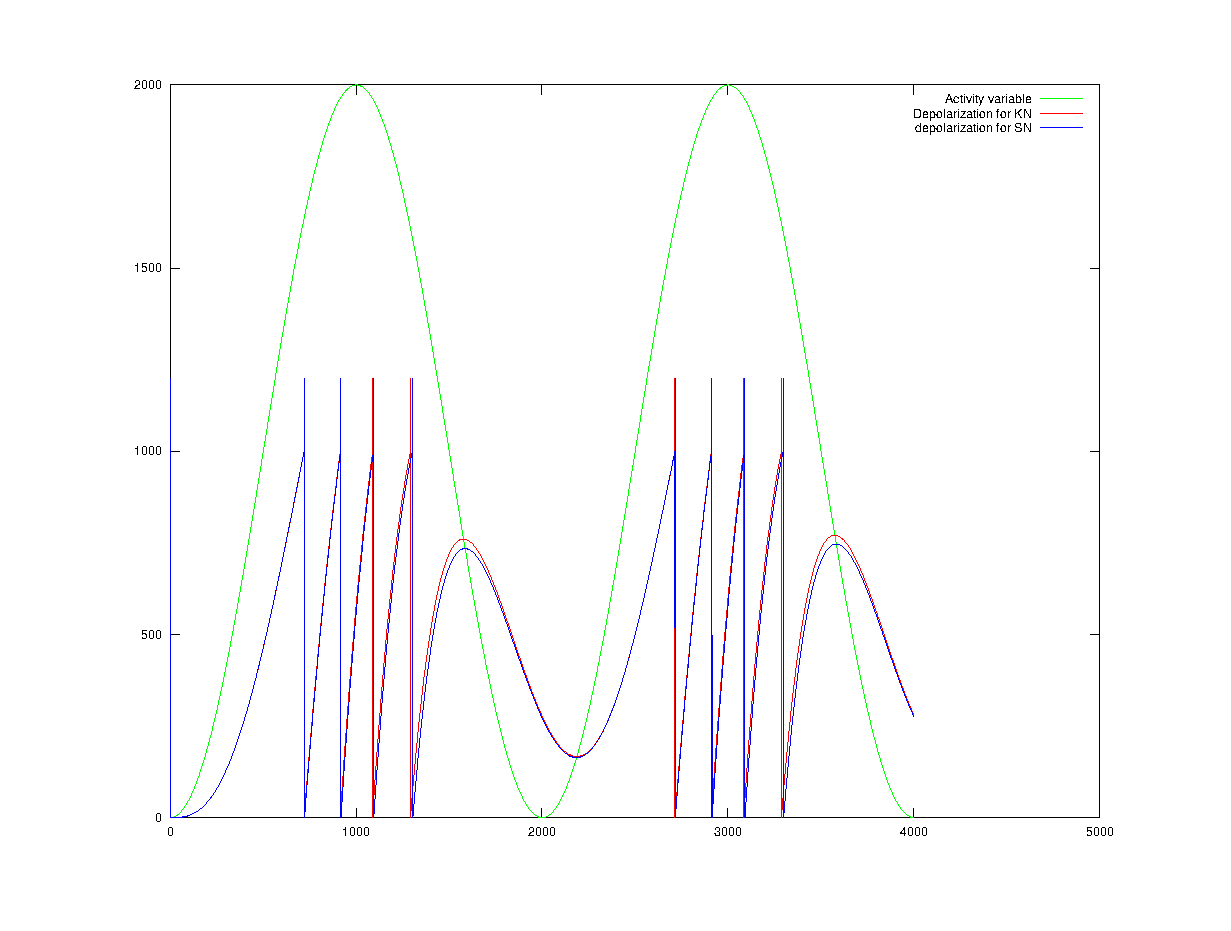
\includegraphics[width=0.95\textwidth]{eps_Comparison_between_the_two_sensors__depol.eps}
	%\end{center}
	\caption{The depolarization curve for a SANN node and a $\kappa$ANN node with the same input. The sensor function is also plotted in green for the analysis of the result.}
	\label{figComparisonBetweenSsensorAndKsensorDepolCurve}
\end{figure}

%The sensor function used for the comparison of the time course of the depolarization of a single node is 
The sensor function used in fig. \ref{figComparisonBetweenSsensorAndKsensorDepolCurve} has the formula \mbox{$f(t) = \tau (1 + cos( \frac{\pi \, t}{1000} ))$}, where $\tau$ is the firing threshold for the neuron. 
The activity variable of the K\_sensor\_auron is set to the value of the sensor funciton every time we iterate time. %XXX i time_class::doTask() Skriv litt meir. 
%For the K\_auron the activity variable is at each time step set to this variable. 
When \emph{time\_class::doTask()} updates the K\_sensor\_auron's activation level, this is done by updating the ``input'' to the dendrite.
%When K\_sensor\_auron changes its activation level, we do this by sending the sensed signal to the dendrite. 
%TODO Neste linje: referer (cite) eller internreferer til annen plass i teksten. Trur det er best å CITE.
This is very simular to the mechanisms of a sensor neuron in biology. %Evt kan eg skrive at "this is strongly inspired by nature".
%referer.
%Beste for refereringa over er nok å skrive om dette i BiologiskeSystemer.tex, og referere til plassen det står. 

%TODO Skriv ENTEN forrige linje ELLER neste greiene. NO: Repeterer meg sjølv! XXX
This implementation is strongly inspired by the biological neural system, and the stimuli is sent to the dendrite as any synaptic input.
For the K\_sensor\_auron this gives the code
%TODO Vær sikker på at dLastSensedValue = dSensedValue; dSensedValue = (*pSensorFunction)();
% Først i koden, under.
%ELLER kanskje heller: skriv om changeKappa_abs() ?!?
\begin{lstlisting}
dLastSensedValue = dSensedValue;
dSensedValue = (*pSensorFunction)();

changeKappa( dSensedValue - dLastSensedValue ); 
\end{lstlisting} %Eller så kan vi gjøre det direkte. (sette Kappa til målt verdi. har impa begge..)
and for the s\_auron we have %TODO BLI HEILT SIKKER PÅ ALPHA. Sjekk om det fortsatt er som under, eller om dette har blitt tatt inn i s_dendrite::newSignal() XXX
\begin{lstlisting}
pInputDendrite->newInputSignal( (*pSensorFunction)() );  
\end{lstlisting} % TODO Forstå greia med ALPHA! (er der fortsatt slik at eg sender inn
							% pInputDendrite->newInputSignal( (*pSensorFunction)() * ALPHA );   XXX ?


Because of the mechanisms implemented for synaptic transmission in $\kappa$ANN is based on the derived, we change $\kappa$ by the discrete variant of the derived; 
The current sensed value minus the last sensed value.% or dSensedValue - dLastSensedValue.
For the s\_auron we incoorporate the time constant T as $\frac{1}{T} = \alpha$ %eller :  $.. = $ ALPHA 
		by sending the above listed input to the s\_sensor\_auron's dendrite.


In figure \ref{figComparisonBetweenSsensorAndKsensorDepolCurve} we can se the results. 
As can be seen, the depolarization of the K\_auron and the s\_auron is quite simular.
There is a small difference between the curves.
%It is hard to know the specific reason for the error in this implementation.  In the following section I will discuss possible explanations.

What is interesting about this curve is that it seems that the depolarization curves follow eachother exactly %Dette er rett stavemåte: exactly (google translate)
for the rising phase of the sensor curve. For the falling phase of the curve we get some difference between the depolarization of the SN and the $\kappa$N.

% Skrive at for SANN så:
For discrete integration we may get something called the trunctation error. The ``local truncation error'' is the immediate error after each time step. 
The ``global truncation error'' is the error following integration multiple local truncation errors. %eller "many truncation errors", eller noke anna? (kan bli for pent språk også!)
The global truncation error is defined as the absolute difference between the approximated solution and the actual solution. 
For the SN this might become a problem, and could be the basis of the difference of the simulated node's depolarization.%Skriv om. XXX

% TODO TODO TODO Skriv også at denne "truncation error" er tatt hand om i KANN, og bude vore minimal. For SANN er ikkje dette mulig (Ingen mulighet å rekalulere verdien).
%  					XXX Dette er veldig viktig poeng for seinere analyse av KANN vs. SANN!

\subsubsection{Trunctation error of the SN} %Kanskje skrive "Spiking Node". Hugs at overskrifta blir også oppført i "index".
In SANN each node is modelled as a leaky-integrate-and-fire neuron.
When the depolarization of the SN is updated, the leak of the neuron calculated as the previous value times the leak constant.
The updated value then becomes %todo Skriv om denne setninga.
\begin{equation} %TODO Introduser denne ligninga tidligare i oppgava. Her skal eg bare skrive siste del av den:    v_t = (1-\alpha) * v_{t-1}  XXX HAR EG GJORT DET? TODO SJEKK!
	v_t =  (1-\alpha) * v_{t-1}  
\end{equation}
%TODO Skriv om: krøtkete måte med/mellom alle komma'ane.
The discretization of the system introduces a small error, the local truncation error, that varies with the size of the time step and the derived of the value function $\dot{v}(t)$. %"local truncation error"

The leak is calculated as the $-\alpha v_{t-1}$.
% Skriv at når feilen oppstår, så er dot(v(t)) positiv, dette gir:
When $\dot{v}(t)$ is positive, $v_{t-1}$ is less than the value $v_t$, varying with the size of the time step and the differentiated value function $\dot{v}(t)$.
When $\dot{v}(t)$ is negative, we get the oposite result.
%skriv at dette nuller ut problemet. (MEN (det kommer at) siden det alltid fyrer etter positiv flanke, blir det integral av en liten integralfeil ved kvar fyring. XXX Viktig poeng. Sjekk at det er stort nok skrevet lenger nede.

Each small error is integrated up to a larger error, the global trunction error. 
If some situation is analyzed where the value is the same as the initial value, the integral of the derived over this interval is per definition zero.
Global trunctation error will then dissapear. 
This further implies that for a continous signal that varies around some working point, the global trunctation error will not diverge.  %google sa at det heite "diverge"

\begin{figure}[hbt!]
	\centering
	%\begin{center}
		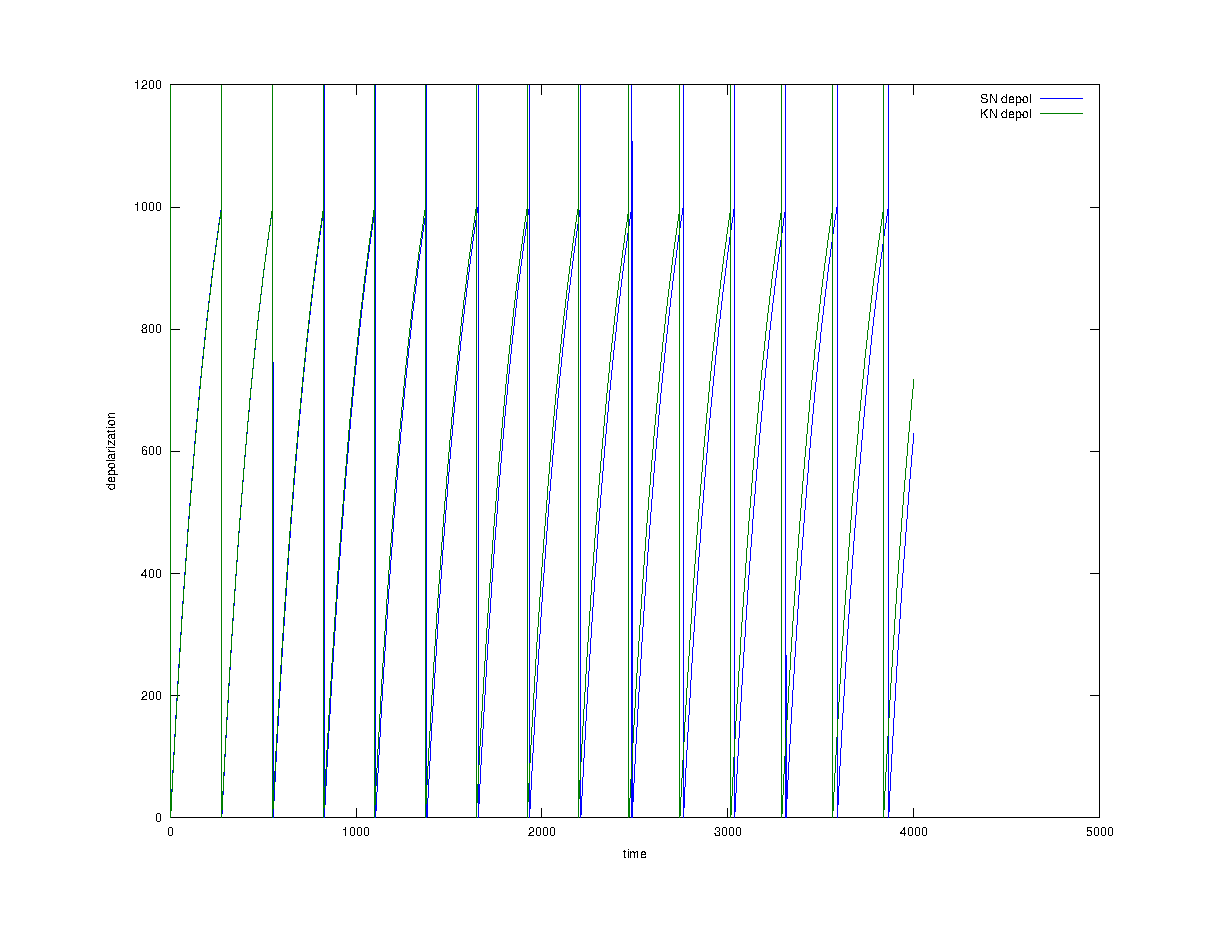
\includegraphics[width=0.95\textwidth]{eps_comparison_between_KN_and_SN_ConstKappa.eps}
	%\end{center}
	\caption{The depolarization curve for a SANN node and a $\kappa$ANN node with the same input. The sensor function has an input equivalent to an activation level of $\kappa = 1.5 \tau$ for both nodes.} %XXX Eller for begge nodeModeller
	\label{figComparisonBetweenSsensorAndKsensorDepolCurveCONStActivityLevel}
\end{figure}

The depolarization of a neuron have a discontinuity when the neuron fires an action potential. 
When the neurons depolarization reaches the firing threshold the value is reset to $v_0 = 0$.
In other words, each time the value of a node reaches a positive threshold, the value is reset.
In this case the global trunctation error will continue to grow, and the difference between the value curves for the SN and the $\kappa$N continues to grow. %TODO Ikkje dette. Skriv heller eit utfall som Stavdahl vil syns er SKUMMELT!

To se if this is the backgound for the error, we isolate the error by giving the sensor aurons a constant sensor function, with an activation level of $\kappa = 1.5 \tau$.

The result is presented in fig. \ref{figComparisonBetweenSsensorAndKsensorDepolCurveCONStActivityLevel}. % .eps
If the previous analysis of the problem is sound, the SN should have a depolarization that is higher than is should be.
This implies than the depolarization curve for the SN would be ``before'' that of the $\kappa$N, which is the opposite of the situation of fig. \ref{figComparisonBetweenSsensorAndKsensorDepolCurveCONStActivityLevel}.

\subsubsection{Rounding errors}
%TODO Skriv om: Ikkje røp løysing først. La det være litt spenning!
After a more thorough analysis of the error, it seems that the difference is an effect of a rounding error.

If we change wievpoint on the error and see the difference between the two cuves as an effect of time, we can say that the $\kappa$N's depolarization curve lies before the SN's depolarization curve.
This implies that the $\kappa$N fires before the SN, and thus starts earlier on the depolarization for the next period.

In many programming languages a float is always ``rounded down''. This means that the DECIMAL %XXX FINN RETT ORD: Det som står etter komma TODO
	is removed from the number, and the integer becomes the same as the integer part of the number.

%TODO Viktig: Hugs å skrive om kvifor eg valte en mindre periode i starten av sensor-funk. Dette er viktig, ellers trur han nok at eg bruker dette for å skjule feilen..
\begin{figure}[hb!tp]
	\centering
		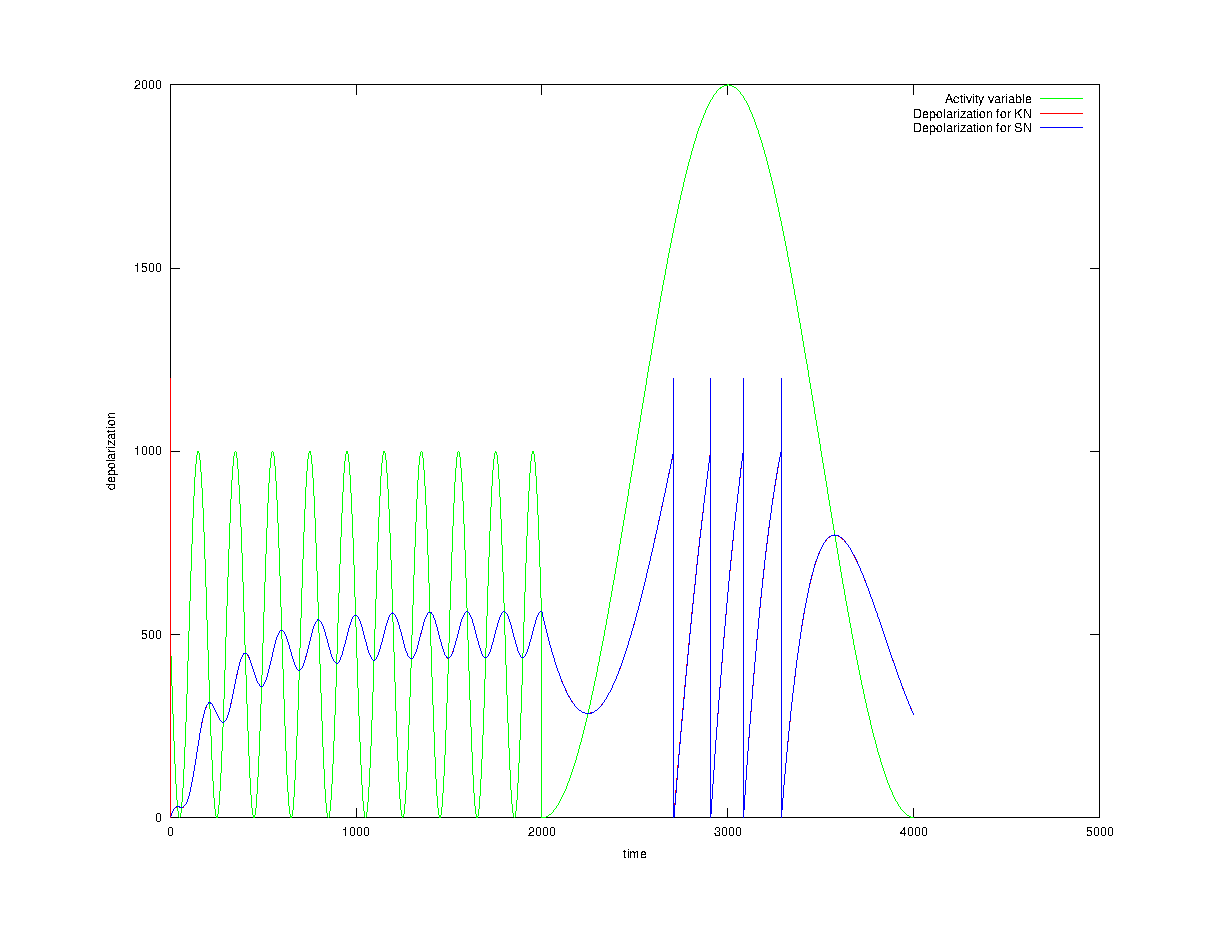
\includegraphics[width=0.95\textwidth]{eps_Comparison_between_the_two_sensors__depol_FIKSA.eps}
	\caption{Comparison between the SN's and $\kappa$N's depolarization curve. The sensor function is plotted in green for analysis purposes.}
	\label{figComparisonBetweenSsensorAndKsensorDepolCurveFIXEdError}
\end{figure}

When the $\kappa$N calculates the estimated firing time, this calculation is done in a double precision floating point number. 
To use this in the scheduler is must first be transformed to an integer variable. When this time step arrives, the task is executed.

%TODO Skriv at vi vil heller runde til nermeste integer, opp om det er best.
% Så skriv korleis dette gjøres, så finn rett kurve.
% TODO analyser frem og tilbake om kor feilen ligger. Det er fortsatt mulig at feilen er for KANN (men trur ikkje det. Legg at feilen er maks når subthreshold polarization er størst. Osv.) XXX
If we instead round to the closest integer, by adding $0.5$ to the float before it is converted into an integer, we get the depolarization curve presented in fig. \ref{figComparisonBetweenSsensorAndKsensorDepolCurveFIXEdError}.
In the improved depolarization curves for the auron, the error is small and can not be seen on the plot.

%Ikkje heilt sikker på om det er heilt rett: størst etter "rising flank of the ..", Bli heilt sikker på dette.
The error is found to be largest right after the rising flank of the activity variable's curve. %TODO ta vekk:   [ , the value of the sensor function. ] ?
For the situation in fig. \ref{figComparisonBetweenSsensorAndKsensorDepolCurveFIXEdError} this is at time t=3000.
At this time iteration the value of the SN is 1.015 more than the value of the $\kappa$N. 

This deviation is substantially smaller that the deviation originating from the rounding error, but it indicates that the analysis made in the previous subsection is correct. %gjør om: ikkje "correct" men kanskje mindre påståelig?
%TODO Skriv analyse av denne feilen, og peik på mulige scenarioer.


% TODO KANSKJE :   \subsection{Floating point calculation pitfalls}
%                  Skriv om mulighetene for feil når man bruker float/double.


% - integralfeil for SN
% - Integralfeilen kommer antagelig av at lekkasjen  
% - For SN vil lekkasjen regnes ut fra verdien ved forrige tissteg. Denne diskretiseringseffekten vil forplante seg i at for positiv derivert av depol-kurva vil SN-depol være litt over, og for negativ flanke : motsatt.
% 		Dette er fordi lekkasjen regnes ut fra forrige verdi, som for stigende flanke er mindre enn den noværande verdien, og vi får en mindre lekkasje => for stor verdi.
% - denne feilen vil nulles ut for eit periodisk signal uten sprang (over en periode vil integralet av positiv flanke og neg. flanke bli null.
% - dersom vi har eit sprang, eller enda verre: eit sprang som alltid ligger etter en viss mengde med pos. flanke, vil vi få summert opp integral-feilen.
% For auronet vil depol settes lik 0 etter en viss mendge pos. flanke for depol. kurva. Dette skaper problemet.

% Eg har også vurdert om det er feil fra implemenasjonen: at de har ulik refraction time, MEN eg trur ikkje dette: 
% 		En slik feil ville vore mindre (eit-to tidssteg per fyring) => ikkje synlig på eit plott over fleire tusen iter's.


% MEN PROBLEMET ER FEIL VEI! JEje. Drit i det!




% Den lille forskjellen mellom s_sensor_auron og K_sensor_auron er noko eg kan skrive mykje om i 'discussion'.
% Eg har tanker om at det er pga. at eg bruker integer (tid) i ligningene, og vi får dermed avrundingsfeil. Litt overraska over at feilen er så liten..
% 	Det er også mulig at den lille forskjellen kommer av forskellane i korleis sensor-funksjonen blir oversatt til depol.
% 		- K_sensor_auron oversetter sensorFunk direkte til aktivitetsVariabel Kappa, mens
% 		- s_sensor_auron sender gir eit enkelt input per tidsiterasjon gitt av ligninga (W_ij / [time constant]), eller  ALPHA * W_ij
%   XXX Dette trenger grundigare analyser!





%XXX Skriv i conclusion:
%Because a network of connected neurons have a large degree of complexity, it is best to start with comparing the depolarization of single nodes.
%For comparison of the two models, we will first compare the depolarization of a single neuron of each model.
%Because a system comprised of a network of neurons have 


\section{Resultat for effektivitetssammenligning}



\section{Discussion}
In the course of this project new model for artificial neural networks have been developed. 
Because the primary focus of the project was to compare a new model for ANN with the ability to represent both firing time and firing frequency, with the SANN model, the development and implementation recieved this focus. 
The new model is therefore implemented as a mere variant of a third generation ANN.
%XXX Kanskje eg overdriver kor liten eg har gjort den :  "... mere variant of ..." Skriv litt mindre høg på pæra?

If we define the third generation ANN as a network of nodes capable of integrating the input to a state for the node, and this state gives the firing time of the node, it is possible to place $\kappa$ANN in this group.
The output of each node in $\kappa$ANN could be defined to be the spikes after a sufficient input to the node.
In this case the ANN becomes a Mealey automata of the SANN model. This is how it is implemented in this project.

If we instead let each $\kappa$N give an output as a function of the present and estimated future input, and give a similar output, the network becomes something else.
The output now varies as a function of the input, and the node becomes stateless in this respect. If desired, the spike time and state of the neuron can still be calculated. 
If the third generation ANN is defined as a network of nodes that gives output as a function of the nodes value, $\kappa$ANN therefore falls outside this group.

In this implementation, it is possible that the full advantage of the new model is neglected in the desire to compare the model to the SANN model.
Because this was first discovered when the results were analyzed, and due to little time, this will be placed under "for furter work". % TODO TA vekk/SKriv om!
%FORTSETT HER!

%så gå over til sammenligning av denne mot SANN.


\section{Discussion 2. Denne skal nok vekk.}

% TODO TODO TODO TODO TODO TODO TODO TODO TODO TODO TODO TODO TODO TODO TODO TODO TODO TODO TODO TODO TODO TODO TODO TODO TODO TODO TODO TODO TODO TODO TODO TODO TODO 
% DETTE er ikkje diskussjon. Dette er implementasjon eller noke. Finn ny plass!
% TODO TODO TODO TODO TODO TODO TODO TODO TODO TODO TODO TODO TODO TODO TODO TODO TODO TODO TODO TODO TODO TODO TODO TODO TODO TODO TODO TODO TODO TODO TODO TODO TODO 

%En eller anna plass: (ikkje akkurat her) Skriver her fordi eg har inspirasjon no, og ikkje vil leite..) 	Ja! Kanskje i "conclutions"XXX
Implementing the mechanisms of a neural simulator is not trivial, even without optimizing it for run time efficiency.
%todo SKriv om neste linje! xxx
Even if this is not an important aspect of this project I have tried to, wherever possible, optimize the implementation for efficiency.
%Skrive kvifor: Om at designet er optimalisert både for generalitet (for å gjøre utvidelser/endring lettere) og for effektivitet. DETTE for å kunne bruke implementationen videre (personlig, eller for andre).

The functions that are most often called are inlined. This means that I have given a hint to the compiler to put the compiled code wherever the functions are called.
This causes the function calls to run faster but also increases the size of the executable file, so this should be used with caution. %Kanskje skrive dette, men også da skrive størrelse på endelig program. ca. 0.5 M (?)
For this implementation, size will not be a problem. %Kvifor?
Inlining of functions are still kept to a minimum, in case of further work on this software. %skriv annaleis. Kvifor "in case of further work on this software."? Forklar bedre, eller skriv om (anna argumentering).

Also in other parts of the implementation, the code is written with a focus on possible future expantion.
%Difor er ting laga enkel å forstå for en som kan nevro: oppsettet av nodene er lagt opp som det biologiske neuronet.
The object model is designed to be general for the two models, both to make the two implementations more comparable for this project and to make the implementation better suitable for future comparison.

The design of each node is based on the biological neuron to be more intuitive for programmers with knowledge of neuroscience. 
This is not only to make the implementation easier to use for potential future programmers, but also because little is known about what is important in neuroscience.
If the implementation is constructed strongly inspired by the emulated system, with multible elements constructed in the same way as the original system, expantion and modification of the indivitual elements involve less effort.
Say, for example, that new aspects are discovered tomorrow. In this case, the code can easier be modified after this discovery.

This principle does not only account for future uses by other programmers.
In multiple occations, aspects that are where new to me have been implemented at after the main functionality of the classes where designed. 
This required less work because I followed principles that was important to Bjarne Stroustrup during the creation of C++; To make the design general and open and suited for any future uses.%ELLER NOKE Siter"TheDesignAndEvolution of C++".


% TODO TODO TODO TODO TODO TODO TODO TODO TODO TODO TODO TODO TODO TODO TODO TODO TODO TODO TODO TODO TODO TODO TODO TODO TODO TODO TODO TODO TODO TODO TODO TODO TODO 
% dette ER diskurs (?) :
One element that is not implemented, is axo--somatic and axo--axonic synases. 
This is synapses where the input to the postsynaptic neuron enters at other places of the neuron than the dendrite. 
In biology, most inhibitory synases have theire input close to the soma of the postsynaptic neuron. 
This will give the inhibitory input less delay compared to the exitatory input, and might be an important aspect in neural computations.
This can be implemented easily if this is found to be important for some future use of this code.

An other important aspect that is not impelented is axo-axonic synapses, linked to short term synaptic plasticity.
%XXX An axo--axonic synapse is a synase that enters the postsynaptic neuron somewhere close to one of its output synapses.
% Gjør om rekkefølgen litt. Skriv om short-term syn.p. først, så evt. axo-axonic synapses.
Short--term synaptic plasticity is synaptic plasticity that does not have any long term effect of the neuroal network (learning), only on more immedate aspects of signal transmission.
In particular, we have the synapses that gives input near the axon terminal of the neuron (axo-axonic synapses). This will alter the depolarization at the neurons output synapses. %og auke/minke mengde Ca2+ i presyn. bit av synapsen.
This will not cause any transmission to occur, only ``prime'' the presynaptic membrane of the synapse for transmission.
When the next action potential arrives, the size of the transmission will be larger than usual (or less, depending on whether the axo--axonic synapse is exitatory or inhibitory).
Again, neither short--term synaptic plasticity or axo--axonic synapses has been implemented because this was not an aspect of this project and due to time constraints.
% Skriv heller at short--term syn.p. ikkje er implementert, så axo-axonic synapses ville ikkje auka funksjonaliteten til simulatoren.
Implementing it will involve less work due to the implementation design in this code.
% Denne setninga er for å vise at det er lett å innføre. Skriv om.

If the goal of the implementation is to simulate a neural network from biology, spatial and temporal resolution is more important than efficiency of the calculation.
%When it comes to temporal and spatial resolution, this can easily be extended.
In this implementation, spatial and temporal resolution can easity be extended.
If we want to increase the accuracy, this can be done by increasing the number of elements in each node (and making the timestep accordingly smaller).
This will also make the computational efficiency of the simulator less, and the pragmatic use of the simulator will suffer.

If we need a better accuracy, and for example double the number of serial elements in each node and halve the size of the timestep, the functioning of each element will be the same.
The temporal and spatial resolution will be increased two-fold at the expence of the computational efficiency of the simulator.

With ``spatial resolution'' i refer to the ability to separate between elements located at different positions in space.
This is important for the output, scince different output synapses are situated at different locations of the neurons axon.
This will cause different transmission delays, and might be important for the neural calculations.
% Also the axon will be have more elements, and different synapses along the axon may have differenti time delay.
This gives us the ability to make a separation between ``early synapses'' and ``late synapses'' along the axon, and gives us a better spatial resolution for the simulated neuron.

The whole reason for developing the third generation ANN, spiking artificial neural networks, was the growing focus on the timing of the different events within the neural network.
This is computational demanding, and high resolution simulations is not suited for real time pragmatic uses of ANNs. For simulations used to test hypothesis in neural science, however, accuracy is most important.
The focus on generality in this implementation will therefore make the code reusable for possible future pragmatic uses and for implementing neural simulators.

If the new model is more effective than the old model for spiking neural networks, we can not know whether this is only goes for one of these uses. 
For this reason I found it best to implement as generally as possible, for future efficiancy comparison between the two models.
%Skrive eksempel: "More specifically, if we divide the axon into smaller pieces, spatial accuracy is better."
%Skriv om forskjellane mellom KANN og SANN. Her kommer kanskje største fordelen med KANN? (Kan kanskje legge inn vilkårlig antall element, til tilsvarende størrelse på 'time step').

%slutt: En eller anna plass: ....


\section{Conclution}
% DET neste er ikkje bra å ha her!
Grunnen for å fokusere på spike time, i utgangspunktet var oppdagelsen av at synapser lærer ved positiv eller negativ vekt-endring etter overføring. 
Hvilken, og kva størrelse er avgjort av når synaptisk overføring kommer i forhold til postsyn. fyring.

Etter litt har man funnet ut at desse mekanismene bare gjelder enkelte synapser, der postsynaptiske neurotransmittor receptors er spenningsavhengig for overføring. 
Med høg depolarisering, dvs lav spenning overføres meir, og bl.a. $Ca^{2+}$ som er viktig for postsynaptisk plastisitet.
"To my knowledge" har det bare blitt funnet en slik neurotransmittor-sensor i biologien. Dette er den glutamatiske NMDA receptoren.
Glutamatisk overføring har vore veldig mykje i fokus for synaptisk overføring, og det er ikkje rart at STDP har fått så veldig høgt fokus %NEI, FAEN! må ikkje argumentere mot oppgaveteksten!


\section{Notater: Kva burde eg gjordt annaleis?}
Burde ikkje bygd de to implementasjonane så lik. (?)
Det er vanskelig å sammenligne de to. For K\_auron kunne eg ivertfall droppa dendrite og kanskje axon.
Jeje - vettafaen eg.

Burde ikkje brukt så mykje tid på pEstimatedTaskTime-lista. Kanskje eg kan argumentere for at dette kan være nyttig, men for dette prosjektet er det tidssløs.


\section{Ting som kanskje er nye}
Skriv litt om optimaliseringa gjordt i SANN. Simulert asynkron tid istedetfor oppdatering kvart tidssteg.

Kalkulering av lekkasje: Kvar gang det kommer nytt input, framfor å gjøre det kvar tidsiterasjon.

\section{Kva burde eg gjordt annerledes?}
Skriv at fokuset mitt i denne implementeringa var å sammenligne de to modellene. Dette gjorde at eg satt opp auronet på eg spesiell, og ikkje-optimal måte.
(Både for effektivitet, men også for implementasjon. Det var kanskje vanskeligere å implementere modellen på måten eg gjorde det, enn nødvendig. Kann trenger bare eit auron, med synapser ut.)
Dette burde eg gjordt annerledes, og både implementering og effektivitet ville vunnet på dette.



% XXX Skriv at resetting til v_r etter AP er ikkje instantaneous. Dette tar også litt tid. For videre arbeid vil også dette bli implementert!

% XXX Skriv at KANN er en mellomting mellom fANN og SANN. Det har muligheten til å kommunisere med begge.
% 		- fANN kan overføre aktivitetsnivået sitt direkte til KANN (Kan sette $\kappa$ = input-fra-fANN) -- Begge veier (KANN: kan få info FRA, og gi info TIL fANN).
% 		- SANN kan overføre aktivitetsnivået sitt indirekte til KANN (KN kann analysere input til $\kappa$. KN kan gi output til SN (direkte))
% Det kan være dette er eit stort bidrag for ANN-verden. Dersom det i tillegg er meir effektivt, så ...




\section{resultat av sammenligning: SANN vs. $\kappa$ANN}
	\section{ The transient course of the auron's depolarization }
	Her skal plott av depolarization legges.

	\section{ Det eg får tida til å sammenligne - implementasjon, effektivitet, ...}
	Skrive at implementasjon er noe vanskeligere for KANN, da det også har med fremtidsutsikter. Dette kan forventes, siden KANN noder kan sees på som implemenasjon av en Mealy automata og SANN en Moore automata av spiking neuron.

	\section{ Mulige aspekt som er nye i denne oppgava }
	I likhet med da eg først utvikla SANN, trudde eg at tidsmodellen min var heilt ny. Det at nodene ikkje ble oppdatert kvar iterasjon, men bare ved "events". Dette er feil. "event--driven simulation of SANN".
	
	Er rimelig sikker på at KANN--modellen er heilt ny. Har ikkje hørt om denne, har ikkje funnet den, alle de professorene eg har snakket med har ikkje hørt om slikt, osv.
	
	Kanskje: Leste at det var vanskelig å estimere fyringstid. Dette blir isåfall løst ved KANN.

	Trur KANN gir muligheten for 'abituary time steps' uten å bruke meir prosessorkraft. I så fall kan dette være stort! Kan gi større oppløsning i forhold til 'spatial resolution' også.
	Fordi KANN beregner bare ved endring av node input, ikkje for alle tidssteg..
	(Dette bør også simuleres, slik at eg får data til å støtte meg på)  	Fy faen, dette er fett isåfall!

	\section{ Konklusjon }


\section{diskusjon}

\bibliography{bibliografi}
%\bibliographystyle{abbrvnat}
\bibliographystyle{plain}
\end{document}

